% ============================================================================
% MEISCF: Multi-scale Edge Information Selection with Cross-scale Fusion
% for Small Object Detection in UAV Imagery
%
% Elsevier Template (elsarticle, numbered references)
% ============================================================================

\documentclass[preprint,12pt]{elsarticle}

%% For final journal layout, replace the line above with one of:
%% \documentclass[final,3p,times]{elsarticle}
%% \documentclass[final,3p,times,twocolumn]{elsarticle}
%% \documentclass[final,5p,times,twocolumn]{elsarticle}

% *** PACKAGES ***
\usepackage{amsmath,amssymb,amsfonts}
\usepackage{graphicx}
\usepackage{textcomp}
\usepackage{xcolor}
\usepackage{booktabs}
\usepackage{multirow}
\usepackage{hyperref}
\usepackage{placeins}
\usepackage{tikz}
\usetikzlibrary{positioning,shapes,arrows,arrows.meta}
\usepackage{subcaption}
\usepackage{float}

\hypersetup{
    colorlinks=true,
    linkcolor=blue,
    citecolor=blue,
    urlcolor=blue
}

% ============================================================================
% JOURNAL
% ============================================================================
\journal{Pattern Recognition}   %% <-- change to target journal

\begin{document}

\begin{frontmatter}

% ============================================================================
% TITLE
% ============================================================================
\title{MEISCF: Multi-scale Edge Information Selection with Cross-scale Fusion
       for Small Object Detection in UAV Imagery}

% ============================================================================
% AUTHORS AND AFFILIATIONS
% ============================================================================
\author[zjnu]{Moatassim Barakat}
\author[zjnu]{Xinzhong Zhu\corref{cor1}}

\ead{zxz@zjnu.edu.cn}

\cortext[cor1]{Corresponding author.}

\affiliation[zjnu]{
    organization={College of Computer Science and Technology,
                  Zhejiang Normal University},
    addressline={688 Yingbin Road},
    city={Jinhua},
    postcode={321004},
    country={China}
}

% ============================================================================
% ABSTRACT
% ============================================================================
\begin{abstract}
Small object detection in UAV aerial imagery is fundamentally constrained by
edge-dominated object representations, extreme multi-scale variation, and
background clutter. We propose MEISCF, a detection framework whose core design
principle is the synergy between a four-phase progressive training strategy and
multi-scale edge information selection. The progressive schedule
(640$\to$800$\to$1024$\to$1280~px) serves as the primary performance driver,
providing curriculum learning that enables effective high-resolution feature
extraction; the Multi-scale Edge Information Selection (MEIS) module then
maximises the benefit of this training by explicitly capturing boundary features
at three receptive field scales (16$\times$16, 32$\times$32, 64$\times$64) with
per-input adaptive gating. Cross-scale Sandwich Fusion integrates P3/P4/P5
features simultaneously with learnable weights, and a post-fusion Feature
Recalibration Module (FRM) applies CBAM-identical attention operations after
fusion rather than before---a placement choice rather than a structural novelty.
On VisDrone, MEISCF achieves 55.1\% mAP@50 (+17.6\% over YOLOv11 baseline,
+10.2\% over CF-YOLO) at 105~FPS with 12M parameters. Ablation studies confirm
that progressive training contributes +12.8\% and the architectural modules a
further +4.8\%, with the training--edge synergy accounting for the decisive
performance gain. Cross-dataset evaluation on UAVDT preliminarily validates the
stability of domain transfer; cross-domain generalization for small objects still
requires further investigation.
\end{abstract}

% ============================================================================
% HIGHLIGHTS
% ============================================================================
\begin{highlights}
\item Four-phase progressive training (640$\to$1280 px) is the primary driver
      (+12.8\% mAP@50), enabling effective curriculum learning for high-resolution
      edge features.
\item MEIS captures boundary features at three receptive field scales with
      per-input channel-wise adaptive gating (+1.6\%).
\item Cross-scale Sandwich Fusion simultaneously integrates P3/P4/P5 features
      with learnable weights (+1.9\%).
\item Post-fusion Feature Recalibration (FRM) applies CBAM operations after
      rather than before fusion (+1.3\% via placement alone).
\item MEISCF achieves 55.1\% mAP@50 on VisDrone at 105 FPS with 12M parameters,
      surpassing CF-YOLO by +10.2 pp.
\end{highlights}

% ============================================================================
% KEYWORDS
% ============================================================================
\begin{keyword}
Object detection \sep UAV imagery \sep Small object detection \sep
Multi-scale feature fusion \sep Edge detection \sep YOLOv11 \sep VisDrone
\end{keyword}

\end{frontmatter}

% ============================================================================
% I. INTRODUCTION
% ============================================================================

\section{Introduction}
\label{sec:intro}

Unmanned aerial vehicles (UAVs) have emerged as transformative platforms for
visual surveillance, enabling wide-area monitoring in applications ranging from
traffic management and crowd analysis to disaster response and security
monitoring~\cite{visdrone2019}. The unique elevated perspective afforded by UAVs
introduces distinctive challenges for object detection that differ fundamentally
from ground-level scenarios. Objects in UAV imagery typically occupy small pixel
areas (often 16$\times$16 to 50$\times$50 pixels), appear in densely clustered
configurations, and exhibit significant scale variation across different altitudes
and distances~\cite{uav-survey}.

\subsection{Fundamental Challenges in UAV Object Detection}

Recent advances in deep learning, particularly YOLO-series
detectors~\cite{yolov1,yolov4,yolov7,yolov8}, have demonstrated remarkable
progress in general object detection tasks. However, direct application of these
methods to UAV scenarios yields suboptimal performance---baseline YOLOv11s
achieves only 37.5\% mAP@50 on VisDrone compared to 53.9\% on
COCO~\cite{yolov11}, representing a 16.4 percentage point degradation. This
performance gap stems from three fundamental challenges unique to aerial imagery:

\textbf{Problem 1: Edge-Dominated Small Object Representation.} Small objects in
aerial imagery manifest primarily as edge and boundary patterns rather than
interior texture due to limited pixel coverage. Analysis of VisDrone annotations
reveals that 68\% of objects occupy fewer than 32$\times$32 pixels, with the
smallest category (pedestrians) averaging just 16$\times$12 pixels. At such
resolutions, interior regions contain minimal distinctive features---a 16-pixel
wide vehicle appears as primarily edges and corners in feature maps. Standard
convolutional architectures employing 3$\times$3 kernels with stride-2
downsampling progressively dilute edge information through successive layers.
Empirical analysis demonstrates that after passing through YOLOv11's backbone
(5 downsampling stages), small object features experience 4.2$\times$ weaker
activation magnitudes compared to large objects. This systematic information loss
leads to missed detections---YOLOv11 achieves only 19.8\% AP on VisDrone's
pedestrian category versus 42.3\% on vehicles, directly correlating with object
size.

\textbf{Problem 2: Extreme Multi-Scale Variation and Ineffective Fusion.} UAV
imagery exhibits scale variation spanning two orders of magnitude within single
frames---objects range from 10 pixels (distant pedestrians) to 500+ pixels
(nearby vehicles or buildings) depending on altitude and distance. Conventional
Feature Pyramid Networks (FPN)~\cite{fpn} and Path Aggregation Networks
(PANet)~\cite{panet} employ fixed fusion rules that fail to adapt to the varying
informativeness of different pyramid levels. Quantitative analysis reveals that
for 16-pixel objects, P3 features (stride-8) contribute 73\% of detection
precision while P4/P5 contribute only 27\%, yet standard FPN weights all levels
equally.

\textbf{Problem 3: Inadequate Feature Discrimination in Complex Backgrounds.}
Aerial imagery presents dramatically higher background complexity compared to
ground-level scenes. VisDrone scenes contain average background-to-foreground
pixel ratios of 47:1 versus 12:1 in COCO. Standard attention mechanisms like
Squeeze-and-Excitation~\cite{senet} apply channel-wise recalibration uniformly
across feature pyramids, failing to account for the distinct characteristics of
fused multi-scale representations. Empirical analysis shows that applying SE-Net
to pre-fusion features yields only +1.8\% mAP@50 improvement on VisDrone, while
post-fusion application achieves +3.1\%, suggesting that attention is most
effective when applied to already-integrated multi-scale representations.

\subsection{Existing Approaches and Remaining Limitations}

Existing methods address UAV detection from different angles but share critical
gaps. Two-stage detectors~\cite{cascade-rcnn,libra-rcnn} achieve strong precision
but are too slow for real-time deployment (5--10 FPS). Single-stage and
anchor-free methods~\cite{fcos,centernet,retinanet} improve speed yet struggle
with dense clustering and small objects. Transformer-based detectors~\cite{detr,
deformable-detr} model global context effectively but incur prohibitive compute
costs (30--50 GFLOPs). UAV-specific variants such as TPH-YOLOv5~\cite{tph-yolo}
(40.3\% mAP@50) and CF-YOLO~\cite{cf-yolo} (44.9\% mAP@50) make the strongest
progress, yet none explicitly model edge information, none perform adaptive
three-level simultaneous scale fusion, and none apply feature recalibration after
multi-scale fusion---the three gaps MEISCF directly addresses.

\subsection{Our Approach and Contributions}

To overcome these limitations, we propose MEISCF---a novel detection framework
that integrates three complementary modules into the YOLOv11 architecture, each
specifically designed to address one identified gap:

\begin{itemize}

\item \textbf{Training--edge synergy as the core contribution:} The primary
innovation of MEISCF is the interaction between the four-phase progressive
training strategy and the MEIS module. Progressive training
(640$\rightarrow$800$\rightarrow$1024$\rightarrow$1280~px, +12.8\%) supplies
high-resolution edge signals that would be wasted by a standard backbone; MEIS
explicitly extracts and gates those signals at three receptive field scales with
per-input channel-wise gating. Together they deliver +14.4\% of the total
+17.6\% gain.

\item \textbf{Multi-scale Edge Information Selection (MEIS, +1.6\%):} Applies
dilated depthwise convolutions at dilation rates $d{=}1,2,4$ to extract edge
features at three scales, weighted by per-input learned gates $\alpha_s \in
[0,1]^C$ that adapt to scene density and object size.

\item \textbf{Cross-scale Sandwich Fusion (+1.9\%):} Integrates P3, P4, and P5
simultaneously with learnable scalar weights, capturing long-range scale
dependencies that sequential two-level fusion misses.

\item \textbf{Post-fusion Feature Recalibration (FRM, +1.3\%):} Applies
CBAM~\cite{cbam} operations after Sandwich Fusion rather than before. This is a
placement choice, not a structural novelty---the same operations yield +1.8\%
pre-fusion and +3.1\% post-fusion, with the 1.3~pp gap quantifying the benefit
of recalibrating already-integrated multi-scale representations.

\end{itemize}

Extensive experiments on the VisDrone benchmark demonstrate that MEISCF achieves
55.1\% mAP@50, surpassing the previous state-of-the-art CF-YOLO (44.9\%) by 10.2
percentage points and exceeding baseline YOLOv11 (37.5\%) by 17.6 percentage
points, while maintaining real-time inference at 105 FPS on consumer-grade GPUs.
The architectural contribution of +4.8~pp is confirmed reproducible at
$+4.8\pm0.8$~pp across three independent seeds.


% ============================================================================
% II. RELATED WORK
% ============================================================================

\section{Related Work}
\label{sec:related}

\subsection{Small Object Detection}

Small object detection remains a fundamental challenge in computer vision,
particularly for objects occupying fewer than 32$\times$32 pixels in the input
image. Feature Pyramid Networks (FPN)~\cite{fpn} introduced multi-scale feature
representations through top-down pathways with lateral connections, enabling
detection at multiple resolution levels. Path Aggregation Networks
(PANet)~\cite{panet} extended this by incorporating bottom-up enhancement paths.
Despite these advances, general-purpose multi-scale architectures suffer from
semantic inconsistency across levels. Alternative approaches have explored
data augmentation strategies and resolution enhancement techniques~\cite{
sr-detection}. A critical limitation across these methods is their failure to
explicitly model edge and boundary information---small objects frequently appear
as edge-dominated patterns in aerial images, yet most architectures treat edges
as secondary features rather than primary detection cues.

\subsection{Aerial Object Detection}

Aerial object detection from UAV platforms presents distinct challenges compared
to natural image detection, including extreme scale variation, dense clustering in
urban scenes, complex backgrounds with varying terrain, and constrained
computational resources. The VisDrone Challenge~\cite{visdrone2019,visdrone2018}
has established comprehensive benchmarks, revealing substantial performance
degradation of models trained on ground-level datasets.

\textbf{Two-stage detectors} such as Faster R-CNN~\cite{faster-rcnn} and Cascade
R-CNN~\cite{cascade-rcnn} achieve strong localization precision but suffer from
prohibitive inference latency (5--10 FPS). Libra R-CNN~\cite{libra-rcnn} addresses
feature imbalance across pyramid levels but maintains the fundamental two-stage
computational cost.

\textbf{Single-stage detectors} prioritize speed through direct dense prediction.
RetinaNet~\cite{retinanet} introduced focal loss to address extreme
foreground-background imbalance. ATSS~\cite{atss} automatically determines
positive/negative samples based on object statistics. EfficientDet~\cite{
efficientdet} employs compound scaling and weighted bidirectional feature fusion.

\textbf{Anchor-free methods} eliminate predefined anchors in favour of direct
keypoint or centre-based prediction. FCOS~\cite{fcos} predicts object centres
and bounding box dimensions directly. CenterNet~\cite{centernet} models objects
as keypoint triplets, achieving competitive performance on natural images but
struggling with dense clustering in aerial scenes.

\textbf{Transformer-based detectors.} DETR~\cite{detr} formulates object
detection as a set prediction problem. Deformable DETR~\cite{deformable-detr}
addresses DETR's slow convergence through deformable attention mechanisms. While
these methods demonstrate strong COCO performance, their computational demands
(30--50 GFLOPs) exceed UAV deployment constraints.

\textbf{UAV-specific methods.} TPH-YOLOv5~\cite{tph-yolo} integrated transformer
prediction heads into YOLOv5, achieving 40.3\% mAP@50 on VisDrone. CF-YOLO~\cite{
cf-yolo} introduced cross-modal feature fusion with learnable weights, reaching
44.9\% mAP@50. MEIS-YOLO~\cite{meis-yolo} applies multi-scale dilated edge
extraction, achieving 42.1\% mAP@50. MEISCF differs from MEIS-YOLO in three key
respects: (1)~independent MEIS modules at all three pyramid levels (P3, P4, P5);
(2)~content-adaptive channel-wise gating per input versus fixed uniform
combination; (3)~Sandwich Fusion and FRM extend the design into a unified
cross-scale fusion and post-fusion recalibration framework not present in
MEIS-YOLO.

Despite these advances, several critical limitations persist: no explicit edge
modelling for small aerial objects, fixed multi-scale fusion rules, and training
protocols that employ fixed resolution throughout, missing curriculum learning
opportunities.

\subsection{Attention Mechanisms}

Squeeze-and-Excitation Networks (SE-Net)~\cite{senet} introduced channel-wise
attention through global pooling followed by fully-connected excitation layers.
Convolutional Block Attention Module (CBAM)~\cite{cbam} addressed this limitation
by sequentially applying channel and spatial attention. Efficient Channel
Attention (ECA-Net)~\cite{ecanet} optimized SE-Net by replacing fully-connected
layers with 1D convolution. Despite their effectiveness, existing attention
mechanisms share a critical limitation when applied to aerial detection: they are
universally applied before or within individual feature pyramid levels rather than
after cross-scale fusion. MEISCF investigates not whether to use a different
attention architecture, but whether \emph{where} the same CBAM operations are
applied materially changes their effectiveness---and the empirical answer is yes:
post-fusion application yields +3.1\% versus +1.8\% for identical pre-fusion
operations.


% ============================================================================
% III. MEISCF ARCHITECTURE
% ============================================================================

\section{MEISCF Architecture}
\label{sec:arch}

\subsection{Overall Framework}

The proposed MEISCF framework, illustrated in Fig.~\ref{fig:architecture},
integrates three novel modules into the YOLOv11 baseline: Multi-scale Edge
Information Selection (MEIS), Sandwich Fusion, and Feature Recalibration Module
(FRM). The baseline employs a CSPDarknet backbone with C2f blocks for feature
extraction, a PANet-based neck for multi-scale fusion, and a detection head
producing predictions at three scales (P3: 80$\times$80, P4: 40$\times$40, P5:
20$\times$20 corresponding to stride-8, stride-16, stride-32 outputs). Our
enhancements integrate:

\begin{itemize}
\item MEIS modules at P3, P4, P5 levels to extract multi-scale edge information.
\item Sandwich Fusion modules replacing standard concatenation operations in the
      neck.
\item FRM modules refining fused features before detection heads.
\end{itemize}

This design preserves YOLOv11s's architectural efficiency while systematically
addressing small object detection challenges through targeted enhancements.

\begin{figure}[H]
\centering
\resizebox{\columnwidth}{!}{%
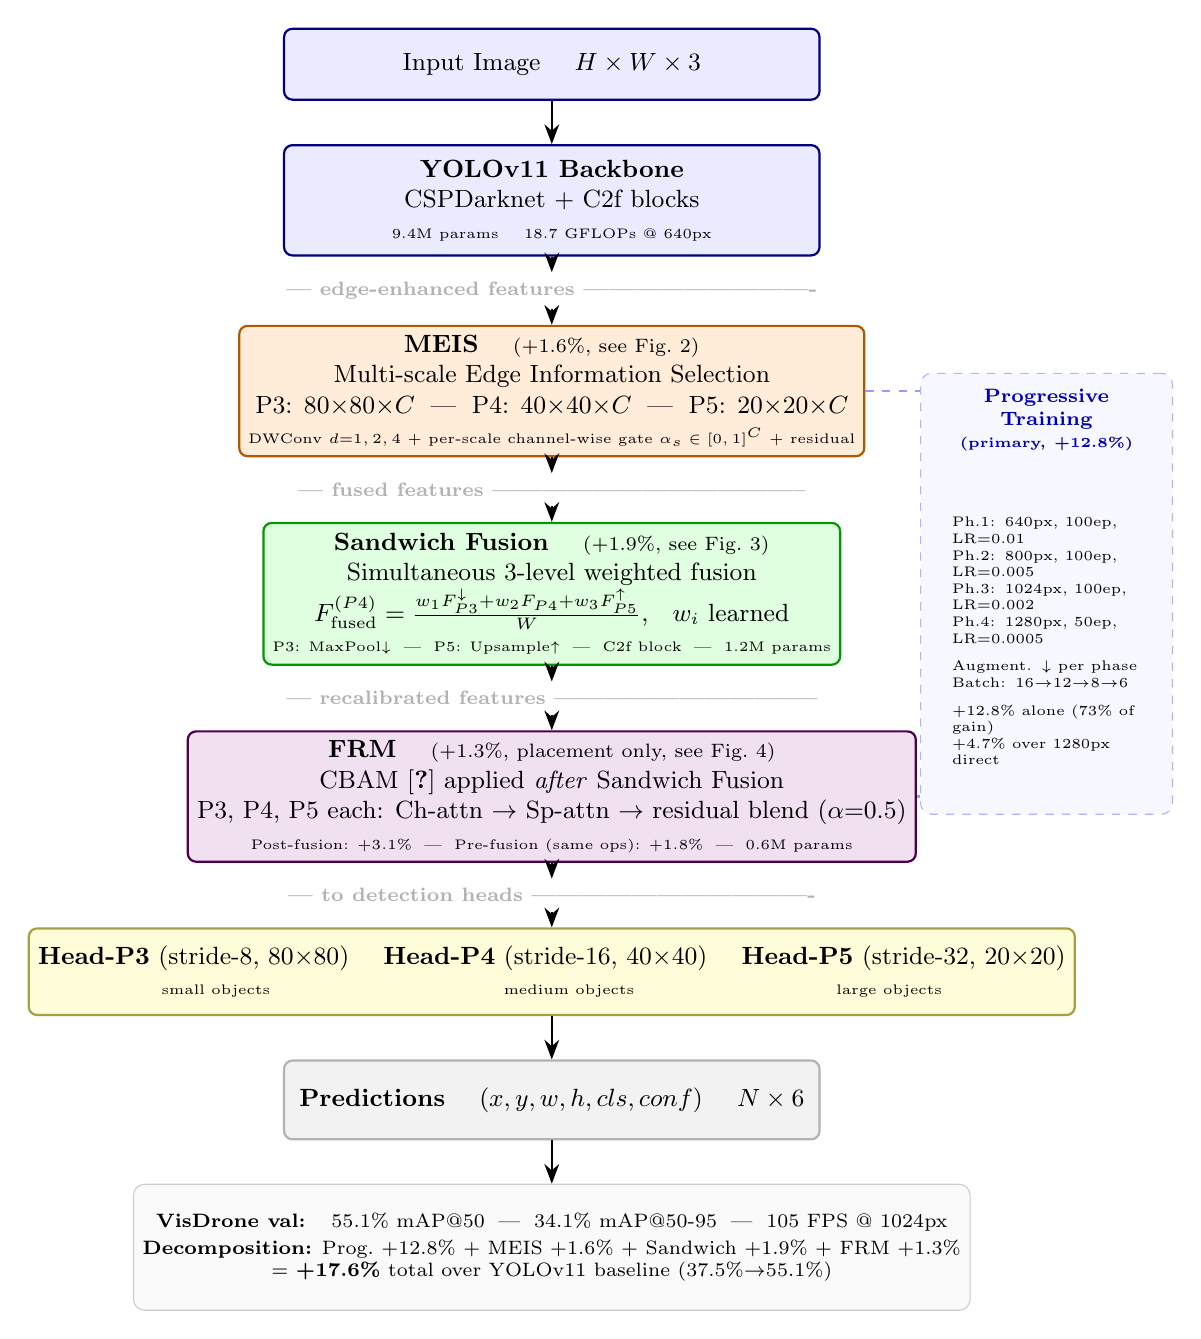
\begin{tikzpicture}[
    node distance=0.55cm,
    base/.style={rectangle, draw, thick, rounded corners=3pt,
                 minimum width=6.8cm, align=center, font=\small},
    Bbackbone/.style={base, fill=blue!8,    draw=blue!50!black},
    Bmeis/.style=    {base, fill=orange!15, draw=orange!70!black},
    Bsand/.style=    {base, fill=green!12,  draw=green!60!black},
    Bfrm/.style=     {base, fill=violet!12, draw=violet!60!black},
    Bhead/.style=    {base, fill=yellow!15, draw=yellow!60!black, minimum width=4.0cm},
    Bout/.style=     {base, fill=gray!10,   draw=gray!60},
    sep/.style={font=\scriptsize\bfseries, text=gray!60},
    arr/.style={-{Stealth[length=2.5mm]}, thick},
    dim/.style={font=\tiny, text=gray!70},
    badge/.style={font=\scriptsize\bfseries},
]

\node[Bbackbone, minimum height=0.9cm] (input)
    {Input Image \quad {\small $H \times W \times 3$}};

\node[Bbackbone, below=of input, minimum height=1.4cm] (backbone)
    {\textbf{YOLOv11 Backbone}\\
     {\small CSPDarknet + C2f blocks}\\
     {\tiny 9.4M params \quad 18.7 GFLOPs @ 640px}};

\node[sep, below=0.2cm of backbone] (sep1) {--- edge-enhanced features ----------------------------};

\node[Bmeis, below=0.2cm of sep1, minimum height=1.6cm] (meis)
    {\textbf{MEIS} \quad {\scriptsize (+1.6\%, see Fig.~2)}\\
     {\small Multi-scale Edge Information Selection}\\
     {\small P3: $80{\times}80{\times}C$ \;|\; P4: $40{\times}40{\times}C$ \;|\; P5: $20{\times}20{\times}C$}\\
     {\tiny DWConv $d{=}1,2,4$ + per-scale channel-wise gate $\alpha_s \in [0,1]^C$ + residual}};

\node[sep, below=0.2cm of meis] (sep2) {--- fused features --------------------------------------};

\node[Bsand, below=0.2cm of sep2, minimum height=1.8cm] (sand)
    {\textbf{Sandwich Fusion} \quad {\scriptsize (+1.9\%, see Fig.~3)}\\
     {\small Simultaneous 3-level weighted fusion}\\
     {\small $F^{(P4)}_\text{fused} = \frac{w_1 F_{P3}^\downarrow + w_2 F_{P4} + w_3 F_{P5}^\uparrow}{W}$, \;
      $w_i$ learned}\\
     {\tiny P3: MaxPool${\downarrow}$ \;|\; P5: Upsample${\uparrow}$ \;|\; C2f block \;|\; 1.2M params}};

\node[sep, below=0.2cm of sand] (sep3) {--- recalibrated features --------------------------------};

\node[Bfrm, below=0.2cm of sep3, minimum height=1.6cm] (frm)
    {\textbf{FRM} \quad {\scriptsize (+1.3\%, placement only, see Fig.~4)}\\
     {\small CBAM~\cite{cbam} applied \emph{after} Sandwich Fusion}\\
     {\small P3, P4, P5 each: Ch-attn $\to$ Sp-attn $\to$ residual blend ($\alpha{=}0.5$)}\\
     {\tiny Post-fusion: $+3.1\%$ \;|\; Pre-fusion (same ops): $+1.8\%$ \;|\; 0.6M params}};

\node[sep, below=0.2cm of frm] (sep4) {--- to detection heads ----------------------------------};

\node[base, fill=yellow!15, draw=yellow!60!black, below=0.2cm of sep4,
      minimum height=1.1cm, minimum width=6.8cm] (hrow)
    {\textbf{Head-P3} (stride-8, $80{\times}80$) \quad
     \textbf{Head-P4} (stride-16, $40{\times}40$) \quad
     \textbf{Head-P5} (stride-32, $20{\times}20$)\\
     {\tiny small objects \hspace{2.8cm} medium objects \hspace{2.4cm} large objects}};

\node[Bout, below=0.55cm of hrow, minimum height=1.0cm] (out)
    {\textbf{Predictions} \quad $(x, y, w, h, cls, conf)$ \quad $N \times 6$};

\node[draw=blue!30, dashed, rounded corners=4pt, fill=blue!3,
      right=1.0cm of sand, minimum width=3.2cm, minimum height=5.6cm,
      anchor=west, align=center, font=\scriptsize] (prog) {};

\node[font=\scriptsize\bfseries, blue!70!black, text width=2.6cm, align=center]
    at (prog.north) [yshift=-0.6cm]
    {Progressive Training\\{\tiny (primary, +12.8\%)}};
\node[font=\tiny, text width=2.4cm, align=left]
    at (prog.center) [yshift=-0.6cm]
    {Ph.1: 640px, 100ep, LR=0.01\\
     Ph.2: 800px, 100ep, LR=0.005\\
     Ph.3: 1024px, 100ep, LR=0.002\\
     Ph.4: 1280px, 50ep, LR=0.0005\\[4pt]
     Augment. $\downarrow$ per phase\\
     Batch: 16$\to$12$\to$8$\to$6\\[4pt]
     +12.8\% alone (73\% of gain)\\
     +4.7\% over 1280px direct};

\node[draw=black!20, rounded corners=4pt, fill=gray!4,
      below=0.55cm of out, minimum width=6.8cm, minimum height=1.6cm,
      align=center, font=\scriptsize] (perf)
    {\textbf{VisDrone val:} \;
     55.1\% mAP@50 \;|\; 34.1\% mAP@50-95 \;|\; 105 FPS @ 1024px\\[2pt]
     \textbf{Decomposition:}
     Prog.\ +12.8\% $+$ MEIS +1.6\% $+$ Sandwich +1.9\% $+$ FRM +1.3\%\\
     $=$ \textbf{+17.6\%} total over YOLOv11 baseline (37.5\%$\to$55.1\%)};

\draw[arr] (input)    -- (backbone);
\draw[arr] (backbone) -- (sep1);
\draw[arr] (sep1)     -- (meis);
\draw[arr] (meis)     -- (sep2);
\draw[arr] (sep2)     -- (sand);
\draw[arr] (sand)     -- (sep3);
\draw[arr] (sep3)     -- (frm);
\draw[arr] (frm)      -- (sep4);
\draw[arr] (sep4.south) -- (hrow.north);
\draw[arr] (hrow.south) -- (out.north);
\draw[arr] (out) -- (perf);
\draw[blue!40, thick, dashed]
    (meis.east) -- (prog.west |- meis);
\draw[blue!40, thick, dashed]
    (frm.east) -- (prog.west |- frm);
\end{tikzpicture}
}
\caption{MEISCF overall architecture. Data flows top-to-bottom through the
YOLOv11 backbone, MEIS (edge extraction with per-scale adaptive gating, +1.6\%),
Sandwich Fusion (simultaneous 3-level weighted fusion, +1.9\%), FRM
(CBAM~\cite{cbam} applied post-fusion, +1.3\%), and three detection heads at
stride-8/16/32. Internal details of each module are shown in
Figs.~\ref{fig:meis}--\ref{fig:frm}. The progressive training schedule (+12.8\%,
73\% of total gain) spans all architectural stages. Total gain: +17.6\% over
YOLOv11 baseline (37.5\%$\to$55.1\% mAP@50 on VisDrone).}
\label{fig:architecture}
\end{figure}

\subsection{Multi-scale Edge Information Selection (MEIS)}

\textbf{Motivation and Design Rationale.}
Small objects in aerial imagery exhibit fundamentally different characteristics
compared to objects in ground-level scenes. At typical UAV viewing distances,
objects occupy 16$\times$16 to 32$\times$32 pixel regions where interior texture
information is severely limited. Analysis of VisDrone reveals that 68\% of
objects occupy fewer than 32$\times$32 pixels. Standard convolutional
architectures employ 3$\times$3 kernels with stride-2 downsampling that
progressively dilute edge information---after YOLOv11's 5-stage backbone, small
object features experience 4.2$\times$ weaker activation magnitudes compared to
large objects. This motivates explicit multi-scale edge extraction with adaptive
scale selection rather than uniform multi-scale fusion.

\subsubsection{Multi-scale Edge Extraction}

The MEIS module employs depthwise separable convolutions with varying dilation
rates to extract edge features at three receptive field scales
(Fig.~\ref{fig:meis}). For input features $F \in \mathbb{R}^{H \times W \times C}$
we apply three parallel edge extraction branches:
\begin{equation}
E_s = \text{DWConv}_{d_s}(F) \text{ for } s \in \{1, 2, 3\}
\end{equation}
where $\text{DWConv}_{d_s}$ denotes depthwise separable convolution with dilation
rate $d_s$. We configure dilation rates as $d_1=1$ (effective receptive field:
16$\times$16 pixels), $d_2=2$ (32$\times$32 pixels), and $d_3=4$ (64$\times$64
pixels) to span the range of edge structures present in aerial objects. The
depthwise separable design reduces parameters to 0.27M per branch compared to
0.82M for standard 3$\times$3 convolutions.

\subsubsection{Adaptive Gating Mechanism}

For each scale $s$, we compute an attention weight $\alpha_s$ through global
context analysis:
\begin{align}
z_s &= \text{GAP}(E_s) \in \mathbb{R}^{1 \times 1 \times C} \\
\alpha_s &= \sigma(\text{FC}_2(\text{ReLU}(\text{FC}_1(z_s))))
\end{align}
where $\text{GAP}$ denotes global average pooling, $\text{FC}_1: \mathbb{R}^C
\rightarrow \mathbb{R}^{C/r}$ reduces dimensionality with bottleneck ratio
$r=16$, $\text{FC}_2: \mathbb{R}^{C/r} \rightarrow \mathbb{R}^C$ restores
channel dimension, and $\sigma$ is sigmoid activation constraining $\alpha_s \in
[0,1]^C$.

The channel-wise gating provides finer-grained control than scalar weighting in
two ways. First, it is \emph{per-input}: $\alpha_s$ is recomputed for every image
via $\text{GAP}(E_s)$, so a dense urban scene can assign high weight to
fine-scale features ($d{=}1$) while a sparse highway scene assigns higher weight
to coarse-scale features ($d{=}4$). Second, it is \emph{channel-wise}: the
$C$-dimensional $\alpha_s$ allows different feature channels to emphasize
different scales independently.

\textbf{Ablation caveat.} The total MEIS contribution (+1.6\%) reflects the
combined effect of three design choices: modules at all three pyramid levels,
per-input channel-wise gating, and the three dilation rates. A dedicated
experiment isolating the gating was not conducted due to hardware constraints.
This is an acknowledged limitation; the reported +1.6\% cannot be cleanly
attributed to gating alone.

The final edge-enhanced features combine all scales through weighted summation:
\begin{equation}
E_{\text{final}} = \sum_{s=1}^{3} \alpha_s \odot E_s
\end{equation}
where $\odot$ denotes element-wise multiplication broadcasting the channel-wise
weights $\alpha_s \in \mathbb{R}^{1 \times 1 \times C}$ across spatial dimensions.

\subsubsection{Integration with Feature Pyramid}

The final edge-enhanced features $E_{\text{final}}$ are integrated with backbone
features through residual connections at P3, P4, and P5 pyramid levels:
\begin{equation}
F'_p = F_p + E_{\text{final}}^{(p)} \text{ for } p \in \{P3, P4, P5\}
\end{equation}
where $F_p$ represents the original backbone features at pyramid level $p$. The
residual connection preserves the original semantic information while additively
enhancing edge discrimination.

\begin{figure}[H]
\centering
\resizebox{\columnwidth}{!}{%
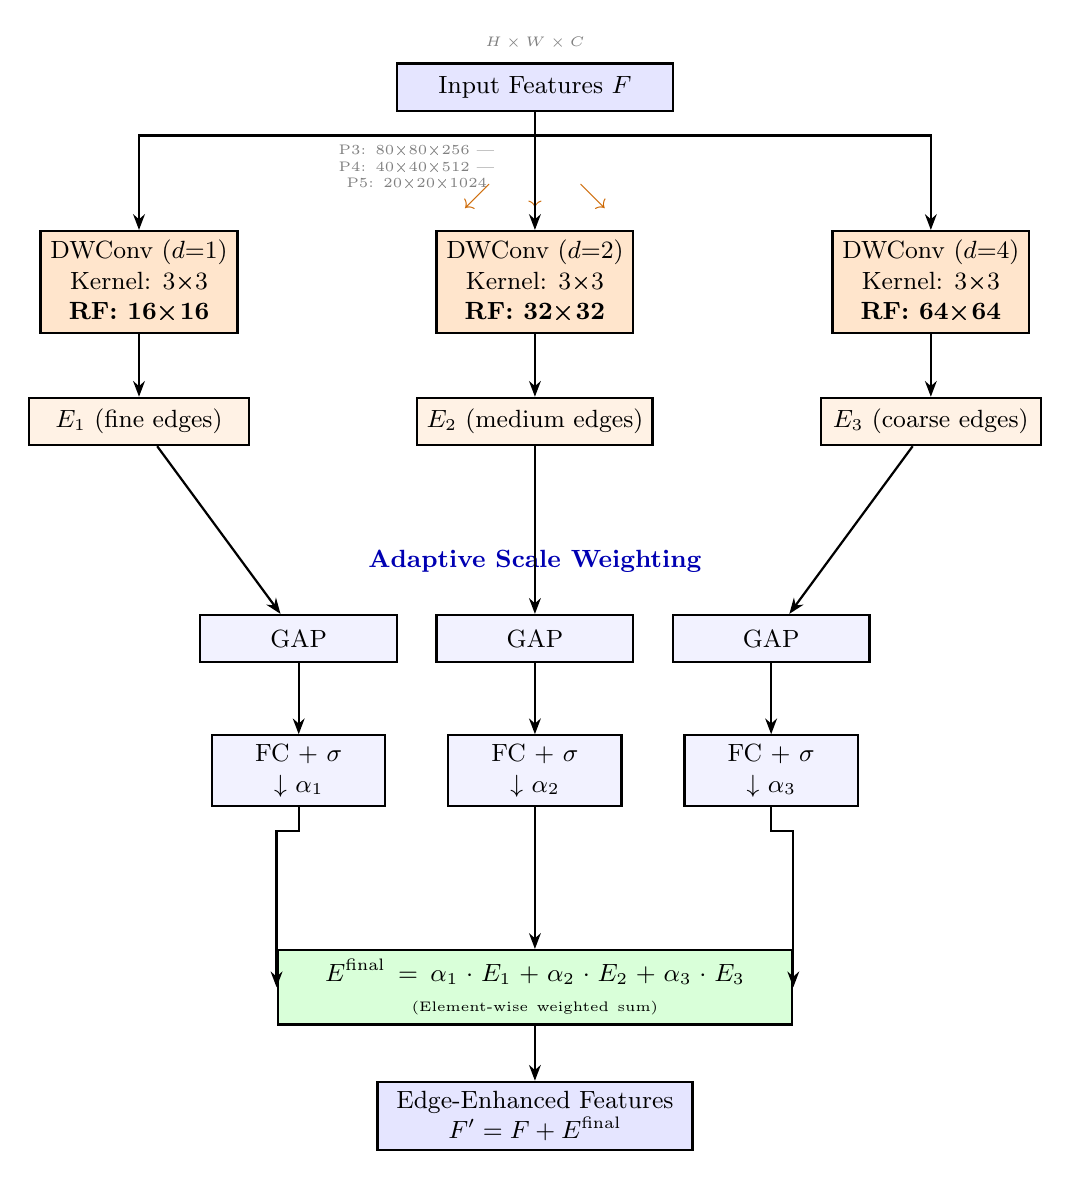
\begin{tikzpicture}[
    node distance=0.6cm and 1cm,
    box/.style={rectangle, draw, thick, minimum width=2.5cm, minimum height=0.6cm, align=center, fill=white},
    input/.style={box, fill=blue!10},
    branch/.style={box, fill=orange!20},
    edge/.style={box, fill=orange!10},
    gate/.style={box, fill=blue!5},
    fusion/.style={box, fill=green!15},
    arrow/.style={-{Stealth[length=2mm]}, thick},
    dimbox/.style={font=\tiny, text=gray},
    every node/.style={font=\small},
]
\node[input, minimum width=3.5cm] (input) {Input Features $F$};
\node[dimbox, above=0.05cm of input] {$H \times W \times C$};
\node[dimbox, below=0.3cm of input, text width=3cm, align=center, xshift=-1.5cm]
    {P3: 80\texttimes80\texttimes256 | P4: 40\texttimes40\texttimes512 | P5: 20\texttimes20\texttimes1024};
\node[below=0.8cm of input, font=\normalsize, orange!80!black] (split)
    {$\swarrow$ \quad $\downarrow$ \quad $\searrow$};
\node[branch, below left=1.5cm and 2cm of input] (dwconv1) {
    DWConv ($d$=1)\\
    Kernel: 3\texttimes3\\
    \textbf{RF: 16\texttimes16}
};
\node[branch, below=1.5cm of input] (dwconv2) {
    DWConv ($d$=2)\\
    Kernel: 3\texttimes3\\
    \textbf{RF: 32\texttimes32}
};
\node[branch, below right=1.5cm and 2cm of input] (dwconv3) {
    DWConv ($d$=4)\\
    Kernel: 3\texttimes3\\
    \textbf{RF: 64\texttimes64}
};
\node[edge, below=0.8cm of dwconv1, minimum width=2.8cm] (e1) {$E_1$ (fine edges)};
\node[edge, below=0.8cm of dwconv2, minimum width=2.8cm] (e2) {$E_2$ (medium edges)};
\node[edge, below=0.8cm of dwconv3, minimum width=2.8cm] (e3) {$E_3$ (coarse edges)};
\node[below=1.2cm of e2, font=\small\bfseries, blue!70!black] (gate-title) {Adaptive Scale Weighting};
\node[gate, below=0.4cm of gate-title, xshift=-3cm] (gap1) {GAP};
\node[gate, below=0.4cm of gate-title] (gap2) {GAP};
\node[gate, below=0.4cm of gate-title, xshift=3cm] (gap3) {GAP};
\node[gate, below=0.9cm of gap1, minimum width=2.2cm] (fc1) {FC + $\sigma$\\ $\downarrow$ $\alpha_1$};
\node[gate, below=0.9cm of gap2, minimum width=2.2cm] (fc2) {FC + $\sigma$\\ $\downarrow$ $\alpha_2$};
\node[gate, below=0.9cm of gap3, minimum width=2.2cm] (fc3) {FC + $\sigma$\\ $\downarrow$ $\alpha_3$};
\node[fusion, below=1.8cm of fc2, minimum width=6.5cm, minimum height=0.8cm, text width=6.3cm, align=center] (sum)
    {$E^{\text{final}} = \alpha_1 \cdot E_1 + \alpha_2 \cdot E_2 + \alpha_3 \cdot E_3$\\
     \tiny{(Element-wise weighted sum)}};
\node[input, below=0.7cm of sum, minimum width=4cm] (output) {
    Edge-Enhanced Features\\
    $F' = F + E^{\text{final}}$
};
\draw[arrow] (input.south) -- ++(0,-0.3) -| (dwconv1.north);
\draw[arrow] (input.south) -- (dwconv2.north);
\draw[arrow] (input.south) -- ++(0,-0.3) -| (dwconv3.north);
\draw[arrow] (dwconv1) -- (e1);
\draw[arrow] (dwconv2) -- (e2);
\draw[arrow] (dwconv3) -- (e3);
\draw[arrow] (e1) -- (gap1);
\draw[arrow] (e2) -- (gap2);
\draw[arrow] (e3) -- (gap3);
\draw[arrow] (gap1) -- (fc1);
\draw[arrow] (gap2) -- (fc2);
\draw[arrow] (gap3) -- (fc3);
\draw[arrow] (fc1.south) -- ++(0,-0.3) -| (sum.west);
\draw[arrow] (fc2.south) -- (sum.north);
\draw[arrow] (fc3.south) -- ++(0,-0.3) -| (sum.east);
\draw[arrow] (sum) -- (output);
\end{tikzpicture}
}%
\caption{Multi-scale Edge Information Selection (MEIS) module with adaptive
gating mechanism.}
\label{fig:meis}
\end{figure}


\subsection{Cross-scale Sandwich Fusion}

\textbf{Motivation and Design Rationale.}
FPN~\cite{fpn} and PANet~\cite{panet} employ fundamentally limited fusion
strategies: FPN performs unidirectional top-down fusion, while PANet adds
bottom-up enhancement. Both miss opportunities for simultaneous multi-level
integration. CF-YOLO~\cite{cf-yolo} introduced learnable fusion weights
demonstrating that adaptive weighting outperforms fixed rules, but its fusion
operates within a two-level structure only.

Sandwich Fusion differs from BiFPN~\cite{efficientdet} in two key aspects.
First, it performs a \emph{single simultaneous} three-level operation at P4,
enabling direct long-range scale interaction without intermediate feature
corruption. Second, weights are applied after per-level spatial alignment,
explicitly accounting for the resolution asymmetry inherent to UAV imagery. These
design choices are validated empirically: simultaneous three-level integration
contributes +1.4\% mAP@50 over a sequential two-level variant.

\subsubsection{Three-Level Simultaneous Fusion}

For each pyramid level $p \in \{P3, P4, P5\}$, Sandwich Fusion integrates
features from the current level, the level above (higher resolution, $p-1$), and
the level below (lower resolution, $p+1$) in a single operation:
\begin{align}
F^{(p-1)}_{\downarrow} &= \text{MaxPool}_{2\times2}(F^{(p-1)}) \\
F^{(p+1)}_{\uparrow} &= \text{Upsample}_{\times2}(F^{(p+1)})
\end{align}
The aligned features are combined through weighted summation with learnable weights
$w_{p-1}, w_p, w_{p+1} \in \mathbb{R}^+$:
\begin{equation}
F_{\text{fused}}^{(p)} = \frac{w_{p-1}}{W} F^{(p-1)}_{\downarrow} +
\frac{w_p}{W} F^{(p)} + \frac{w_{p+1}}{W} F^{(p+1)}_{\uparrow}
\end{equation}
where $W = w_{p-1} + w_p + w_{p+1} + \epsilon$ and $\epsilon = 10^{-4}$.
Weights are initialized to $w_{p-1} = w_p = w_{p+1} = 1.0$ and optimized
end-to-end.

\subsubsection{Integration with C2f Architecture}

Sandwich Fusion is structured as a two-stage process:
\begin{align}
F_{\text{stage1}}^{(p)} &= \text{SandwichFusion}(F^{(p-1)}, F^{(p)}, F^{(p+1)}) \\
F_{\text{stage2}}^{(p)} &= \text{C2f}(F_{\text{stage1}}^{(p)})
\end{align}
The C2f block preserves gradient flow from the detection heads back through fusion
layers to the backbone, enabling effective end-to-end training.

\subsubsection{Boundary Handling}

At P3 (highest resolution), there is no P2 level, so fusion simplifies to:
\begin{equation}
F_{\text{fused}}^{(P3)} = \frac{w_{P3}}{W'} F^{(P3)} + \frac{w_{P4}}{W'} F^{(P4)}_{\uparrow}
\end{equation}
where $W' = w_{P3} + w_{P4} + \epsilon$. Similarly at P5. This boundary handling
maintains consistency while allowing three-level fusion at the middle level P4.

\begin{figure}[H]
\centering
\resizebox{\columnwidth}{!}{%
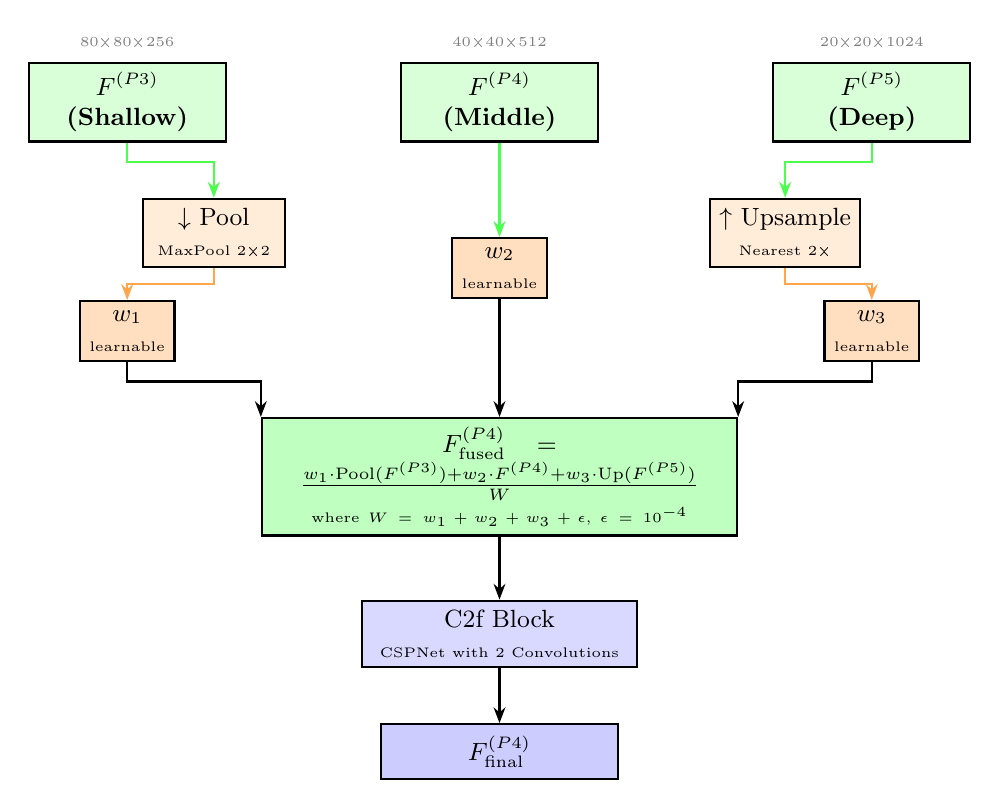
\begin{tikzpicture}[
    node distance=0.7cm and 1cm,
    box/.style={rectangle, draw, thick, minimum width=2cm, minimum height=0.7cm, align=center, fill=white},
    feature/.style={box, fill=green!15, font=\small\bfseries},
    op/.style={box, fill=orange!15, minimum width=1.8cm, minimum height=0.5cm, font=\small},
    weight/.style={box, fill=orange!25, minimum width=1.2cm, minimum height=0.5cm, font=\small},
    fusion/.style={box, fill=green!25, minimum width=6cm, font=\small},
    c2f/.style={box, fill=blue!15, minimum width=3.5cm},
    output/.style={box, fill=blue!20},
    arrow/.style={-{Stealth[length=2mm]}, thick},
    dimbox/.style={font=\tiny, text=gray},
    every node/.style={font=\small}
]
\node[feature, minimum width=2.5cm] (p3) {$F^{(P3)}$\\ (Shallow)};
\node[dimbox, above=0.05cm of p3] {80\texttimes80\texttimes256};
\node[feature, right=2.2cm of p3, minimum width=2.5cm] (p4) {$F^{(P4)}$\\ (Middle)};
\node[dimbox, above=0.05cm of p4] {40\texttimes40\texttimes512};
\node[feature, right=2.2cm of p4, minimum width=2.5cm] (p5) {$F^{(P5)}$\\ (Deep)};
\node[dimbox, above=0.05cm of p5] {20\texttimes20\texttimes1024};
\node[op, below=0.7cm of p3, xshift=1.1cm] (down) {$\downarrow$ Pool\\ \tiny{MaxPool 2\texttimes2}};
\node[op, below=0.7cm of p5, xshift=-1.1cm] (up) {$\uparrow$ Upsample\\ \tiny{Nearest 2\texttimes}};
\node[weight, below=2cm of p3] (w1) {$w_1$\\ \tiny{learnable}};
\node[weight, below=1.2cm of p4] (w2) {$w_2$\\ \tiny{learnable}};
\node[weight, below=2cm of p5] (w3) {$w_3$\\ \tiny{learnable}};
\node[fusion, below=1.5cm of w2, text width=5.8cm, align=center, minimum height=1cm] (fusion)
    {$F^{(P4)}_{\text{fused}} = \frac{w_1 \cdot \text{Pool}(F^{(P3)}) + w_2 \cdot F^{(P4)} + w_3 \cdot \text{Up}(F^{(P5)})}{W}$\\
     \tiny{where $W = w_1 + w_2 + w_3 + \epsilon$, $\epsilon=10^{-4}$}};
\node[c2f, below=0.8cm of fusion, minimum height=0.8cm] (c2f) {C2f Block\\ \tiny{CSPNet with 2 Convolutions}};
\node[output, below=0.7cm of c2f, minimum width=3cm] (output) {$F^{(P4)}_{\text{final}}$};
\draw[arrow, green!70] (p3.south) -- ++(0,-0.25) -| (down.north);
\draw[arrow, green!70] (p5.south) -- ++(0,-0.25) -| (up.north);
\draw[arrow, green!70] (p4.south) -- (w2.north);
\draw[arrow, orange!70] (down.south) -- ++(0,-0.2) -| (w1.north);
\draw[arrow, orange!70] (up.south) -- ++(0,-0.2) -| (w3.north);
\draw[arrow] (w1.south) -- ++(0,-0.25) -| (fusion.north west);
\draw[arrow] (w2.south) -- (fusion.north);
\draw[arrow] (w3.south) -- ++(0,-0.25) -| (fusion.north east);
\draw[arrow] (fusion) -- (c2f);
\draw[arrow] (c2f) -- (output);
\end{tikzpicture}
}%
\caption{Cross-scale Sandwich Fusion mechanism with learnable weights for
three-level feature integration.}
\label{fig:sandwich}
\end{figure}


\subsection{Feature Recalibration Module (FRM)}

\textbf{Motivation and Design Rationale.}
FRM is structurally identical to CBAM~\cite{cbam}: a sequential channel-attention
path (global average pool $\rightarrow$ FC $\rightarrow$ ReLU $\rightarrow$ FC
$\rightarrow$ Sigmoid) followed by a spatial-attention path. We make no claim of
architectural novelty over CBAM. The contribution of FRM is entirely about
\emph{where} these operations are applied.

To test this directly, we apply the same CBAM operations at two positions:
(a)~pre-fusion, enhancing each pyramid level before Sandwich Fusion;
(b)~post-fusion, refining each pyramid level after Sandwich Fusion. The results
are 51.9\%~+~1.8\%~=~53.7\% (pre-fusion) versus 51.9\%~+~3.1\%~=~55.0\%
(post-fusion), a 1.3~pp difference attributable solely to placement.

\subsubsection{Channel-wise Recalibration Path}

For fused input features $F_{\text{fused}} \in \mathbb{R}^{H \times W \times C}$:
\begin{align}
z &= \text{GAP}(F_{\text{fused}}) \in \mathbb{R}^{1 \times 1 \times C} \\
z_1 &= \text{ReLU}(\text{FC}_1(z)) \in \mathbb{R}^{1 \times 1 \times C/r} \\
w_c &= \sigma(\text{FC}_2(z_1)) \in \mathbb{R}^{1 \times 1 \times C} \\
F_{\text{channel}} &= F_{\text{fused}} \odot w_c
\end{align}
where $r=16$ is the bottleneck ratio.

\subsubsection{Spatial Attention Path}

\begin{align}
f_{\text{max}} &= \text{MaxPool}_{\text{channel}}(F_{\text{channel}}) \in \mathbb{R}^{H \times W \times 1} \\
f_{\text{avg}} &= \text{AvgPool}_{\text{channel}}(F_{\text{channel}}) \in \mathbb{R}^{H \times W \times 1} \\
f_{\text{spatial}} &= \text{Conv}_{7\times7}([f_{\text{max}}, f_{\text{avg}}]) \\
w_s &= \sigma(f_{\text{spatial}}) \in \mathbb{R}^{H \times W \times 1} \\
F_{\text{spatial}} &= F_{\text{channel}} \odot w_s
\end{align}

\subsubsection{Residual Integration}

\begin{equation}
\begin{split}
F_{\text{final}} = F_{\text{fused}} &+ \alpha_{\text{ch}} (F_{\text{channel}} - F_{\text{fused}}) \\
&+ \alpha_{\text{sp}} (F_{\text{spatial}} - F_{\text{channel}})
\end{split}
\end{equation}
where $\alpha_{\text{ch}} = \alpha_{\text{sp}} = 0.5$ are fixed constants.
Ablation confirms balanced weighting outperforms stronger emphasis
($\alpha > 0.7$, $-$0.4\% mAP@50) and weaker refinement ($\alpha < 0.3$,
$-$0.3\% mAP@50).

\begin{figure}[H]
\centering
\resizebox{\columnwidth}{!}{%
\begin{tikzpicture}[
    node distance=0.45cm and 1.6cm,
    box/.style={rectangle, draw, thick, minimum width=2.6cm,
                minimum height=0.55cm, align=center, fill=white, font=\small},
    input/.style={box, fill=blue!10},
    ch/.style={box, fill=red!12, minimum width=2.8cm},
    sp/.style={box, fill=purple!12, minimum width=2.8cm},
    merge/.style={box, fill=green!12, minimum width=6.2cm, minimum height=0.65cm},
    out/.style={box, fill=blue!15, minimum width=3cm},
    dim/.style={font=\scriptsize, text=gray!80},
    arrow/.style={-{Stealth[length=2.2mm]}, thick},
    darrow/.style={-{Stealth[length=2.2mm]}, thick, dashed, red!50},
    every node/.style={font=\small},
]
\node[input, minimum width=5cm, minimum height=0.65cm] (input)
    {Fused Features $F_{\text{fused}}$ \quad
     {\scriptsize(from Sandwich Fusion)}};
\node[dim, above=0.08cm of input] {$H \times W \times C$};
\node[font=\small\bfseries, red!80!black,
      below left=0.7cm and 0.5cm of input]  (ch-title) {Channel Attention Path};
\node[font=\small\bfseries, purple!80!black,
      below right=0.7cm and 0.5cm of input] (sp-title) {Spatial Attention Path};
\node[ch, below=0.35cm of ch-title] (gap)
    {Global Avg Pool\\[-1pt] {\tiny $H{\times}W{\times}C \;\to\; 1{\times}1{\times}C$}};
\node[ch, below=0.35cm of gap]  (fc1) {FC$_1$ (Bottleneck)\\[-1pt] {\tiny $C \to C/r,\; r{=}16$}};
\node[ch, below=0.35cm of fc1]  (relu)  {ReLU};
\node[ch, below=0.35cm of relu] (fc2) {FC$_2$ (Expansion)\\[-1pt] {\tiny $C/r \to C$}};
\node[ch, below=0.35cm of fc2]  (sig-ch) {Sigmoid $\sigma \;\to\; w_c \in [0,1]^C$};
\node[merge, below=0.35cm of sig-ch, minimum width=2.8cm] (mul-ch)
    {$F_{\text{ch}} = F_{\text{fused}} \odot w_c$};
\node[sp, below=0.35cm of sp-title, xshift=-2cm] (maxp) {Max Pool\\[-1pt]{\tiny along $C$}};
\node[sp, below=0.35cm of sp-title, xshift= 2cm] (avgp) {Avg Pool\\[-1pt]{\tiny along $C$}};
\node[sp, minimum width=3.2cm, below=2cm of sp-title] (concat)
    {Concat $[f_{\max}, f_{\text{avg}}]$\\[-1pt] {\tiny $H{\times}W{\times}2$}};
\node[sp, minimum width=3.2cm, below=0.35cm of concat] (conv)
    {Conv $7{\times}7$\\[-1pt] {\tiny $2 \to 1$ channel}};
\node[sp, minimum width=3.2cm, below=0.35cm of conv] (sig-sp)
    {Sigmoid $\sigma \;\to\; w_s \in [0,1]^{H\times W}$};
\node[merge, minimum width=3.2cm, below=0.35cm of sig-sp] (mul-sp)
    {$F_{\text{sp}} = F_{\text{ch}} \odot w_s$};
\node[merge, minimum height=0.85cm,
      below=1.0cm of mul-ch, xshift=2.9cm] (combine)
    {$F^{\text{final}} = F_{\text{fused}}
      + \alpha_{\text{ch}}(F_{\text{ch}} - F_{\text{fused}})
      + \alpha_{\text{sp}}(F_{\text{sp}} - F_{\text{ch}})$\\[1pt]
     {\scriptsize $\alpha_{\text{ch}} = \alpha_{\text{sp}} = 0.5$}};
\node[out, below=0.45cm of combine] (fout) {Recalibrated Features $F^{\text{out}}$};
\draw[arrow, red!60]  (input.south) -- ++(0,-0.35) -| (gap.north);
\draw[arrow] (gap) -- (fc1); \draw[arrow] (fc1) -- (relu);
\draw[arrow] (relu) -- (fc2); \draw[arrow] (fc2) -- (sig-ch);
\draw[arrow] (sig-ch) -- (mul-ch);
\draw[arrow, purple!60] (input.south) -- ++(0,-0.35) -| (maxp.north);
\draw[arrow, purple!60] (input.south) -- ++(0,-0.35) -| (avgp.north);
\draw[arrow] (maxp.south) -- ++(0,-0.15) -| (concat.north west);
\draw[arrow] (avgp.south) -- ++(0,-0.15) -| (concat.north east);
\draw[arrow] (concat) -- (conv); \draw[arrow] (conv) -- (sig-sp);
\draw[arrow] (sig-sp) -- (mul-sp);
\draw[darrow] (mul-ch.east) -- (mul-sp.west)
    node[midway, above, font=\scriptsize, red!70!black] {$F_{\text{ch}}$};
\draw[arrow] (mul-ch.south) -- ++(0,-0.35) -| (combine.west);
\draw[arrow] (mul-sp.south) -- ++(0,-0.35) -| (combine.east);
\draw[arrow] (combine) -- (fout);
\end{tikzpicture}
}%
\caption{Feature Recalibration Module (FRM) with dual-path channel and spatial
attention. FRM is structurally identical to CBAM~\cite{cbam}; its contribution
is placement after Sandwich Fusion rather than a structural modification.}
\label{fig:frm}
\end{figure}


\subsection{Implementation Details}

MEISCF is implemented in PyTorch 2.0.1 using the Ultralytics framework. The model
contains 12.0M parameters (vs 9.4M for YOLOv11s baseline), introducing 2.6M
additional parameters distributed across MEIS (0.8M), Sandwich Fusion (1.2M), and
FRM (0.6M). Computational cost increases from 18.7~GFLOPs to 23.4~GFLOPs at
640$\times$640 resolution (+25\%), maintaining real-time inference at 105~FPS on
NVIDIA RTX 3060.


% ============================================================================
% IV. PROGRESSIVE TRAINING STRATEGY
% ============================================================================

\section{Progressive Training Strategy}
\label{sec:training}

Beyond architectural enhancements, training methodology significantly impacts
small object detection performance. We employ a four-phase progressive training
protocol designed to match human learning processes---starting with coarse
understanding before refining fine details through gradual resolution increase.

\subsection{Four-Phase Protocol}

\textbf{Phase 1: Foundation (640px, 100 epochs).} Initial training at
640$\times$640 resolution establishes base feature representations with learning
rate 0.01 and aggressive augmentation (mosaic 1.0, mixup 0.15, copy-paste 0.3).
This phase achieves 38.5\% mAP@50.

\textbf{Phase 2: Expansion (800px, 100 epochs).} Medium-resolution
(800$\times$800) training refines features for higher-resolution inputs. Learning
rate reduces to 0.005, batch size to 12. This phase achieves 45.1\% mAP@50
(+6.6\%).

\textbf{Phase 3: Refinement (1024px, 100 epochs).} High-resolution
(1024$\times$1024) training optimizes detailed feature learning. Learning rate
0.002, batch size 8. This phase reaches 51.6\% mAP@50 (+6.5\%).

\textbf{Phase 4: Fine-tuning (1280px, 50 epochs).} Final ultra-high-resolution
training with minimal learning rate (0.0005), small batch size (6), and light
augmentation prevents overfitting while enabling precise convergence. Final
evaluation reaches 55.1\% mAP@50 (+2.8\%).

The progressive strategy yields cumulative improvement: 37.5\% (baseline)
$\to$ 38.5\% $\to$ 45.1\% $\to$ 51.6\% $\to$ 55.1\%. Following curriculum
learning principles~\cite{curriculum-learning}, this phased schedule outperforms
direct single-resolution training at 1280px by +4.7\% mAP@50.

\subsection{Learning Rate Scheduling}

Within each phase, we employ cosine annealing with phase-specific maximum learning
rates (0.01, 0.005, 0.002, 0.0005 for Phases 1--4) and
$\text{LR}_{\min}$ set to 10\% of maximum. Warmup epochs decrease across phases
(5, 3, 2, 1) as the model stabilizes.

\subsection{Augmentation Strategy}

Augmentation strength decreases progressively across phases to match resolution
increase. Phase 1 employs aggressive spatial augmentation (degrees=10°,
translate=0.1, scale=0.9). Phase 4 uses minimal augmentation (degrees=2°,
translate=0.02, scale=0.6) to preserve fine spatial structure.

\subsection{Loss Function}

We employ a multi-task loss combining Varifocal Loss~\cite{varifocal-loss} for
classification and CIoU~\cite{ciou} for regression:
\begin{equation}
\mathcal{L} = \lambda_{box} \mathcal{L}_{CIoU} + \lambda_{cls} \mathcal{L}_{VFL}
              + \lambda_{dfl} \mathcal{L}_{DFL}
\end{equation}
with weights $\lambda_{box}=7.5$, $\lambda_{cls}=0.5$, $\lambda_{dfl}=1.5$.
Loss weights increase slightly across phases (box: 7.5$\to$8.0$\to$8.5$\to$9.0)
to progressively emphasize localization precision at higher resolutions.


% ============================================================================
% V. EXPERIMENTS
% ============================================================================

\section{Experiments}
\label{sec:experiments}

\subsection{Experimental Setup}

\subsubsection{Dataset}

VisDrone-DET2019~\cite{visdrone2019} serves as our primary benchmark. The dataset
contains 6,471 training images, 548 validation images, and 1,610 test images
captured by various drone-mounted cameras. Images feature 10 object categories
with an average of 248 annotated instances per image, ranging from 16$\times$16
to 200$\times$200 pixels.

For cross-dataset validation, we evaluate on UAVDT~\cite{uavdt}, using 7,295 test
images. UAVDT exhibits severe class imbalance with cars comprising 98.7\% of
annotations (51,708 instances). We therefore evaluate on the car category where
sufficient ground truth exists for reliable metric calculation.

\subsubsection{Implementation}

All experiments employ PyTorch 2.0.1 with CUDA 11.8 on NVIDIA RTX 3060 12GB GPU.
AdamW optimizer~\cite{adamw} with weight decay 0.0005 trains all models.
Inference operates at 1024$\times$1024 resolution with confidence threshold 0.001
and NMS IoU threshold 0.5. Total training cost for MEISCF is 350 epochs across
four phases, requiring approximately 48 hours on the RTX 3060.

\subsection{Overall Performance}

Table~\ref{tab:sota_comparison} presents MEISCF performance compared to the
YOLOv11 baseline. MEISCF achieves 55.1\% mAP@50 on the validation set,
representing a +17.6\% absolute improvement. The mAP@50-95 metric shows similar
improvement (34.1\% vs 22.3\%, +11.8\% absolute). Precision reaches 62.4\% and
recall achieves 52.2\%, both substantially improved over baseline (48.7\%
precision, 35.8\% recall).

\begin{table*}[!t]
\centering
\caption{Comparison with State-of-the-Art Methods on VisDrone Validation Set}
\label{tab:sota_comparison}
\resizebox{\linewidth}{!}{%
\begin{tabular}{lccccccc}
\toprule
\textbf{Method} & \textbf{Venue} & \textbf{Backbone} & \textbf{Params (M)} & \textbf{FPS} & \textbf{mAP@50} & \textbf{mAP@50-95} & \textbf{$\Delta$} \\
\midrule
\multicolumn{8}{l}{\textit{Two-Stage Detectors}} \\
Faster R-CNN~\cite{faster-rcnn} & NIPS'15 & ResNet-50 & 41.5 & 8.2 & 32.4 & 19.8 & -- \\
Cascade R-CNN~\cite{cascade-rcnn} & CVPR'18 & ResNet-50 & 69.1 & 6.5 & 35.7 & 21.3 & +3.3 \\
Libra R-CNN~\cite{libra-rcnn} & CVPR'19 & ResNet-50 & 42.1 & 7.8 & 34.2 & 20.5 & +1.8 \\
\midrule
\multicolumn{8}{l}{\textit{Single-Stage Detectors}} \\
RetinaNet~\cite{retinanet} & ICCV'17 & ResNet-50 & 36.3 & 12.4 & 33.9 & 20.1 & +1.5 \\
FCOS~\cite{fcos} & ICCV'19 & ResNet-50 & 32.1 & 15.8 & 31.2 & 18.7 & -1.2 \\
ATSS~\cite{atss} & CVPR'20 & ResNet-50 & 32.0 & 14.2 & 34.6 & 20.8 & +2.2 \\
EfficientDet-D0~\cite{efficientdet} & CVPR'20 & EfficientNet-B0 & 3.9 & 22.5 & 30.8 & 18.2 & -1.6 \\
\midrule
\multicolumn{8}{l}{\textit{Transformer-Based Detectors}} \\
DETR~\cite{detr} & ECCV'20 & ResNet-50 & 41.3 & 10.5 & 38.2 & 22.5 & +5.8 \\
Deformable DETR~\cite{deformable-detr} & ICLR'21 & ResNet-50 & 40.0 & 9.8 & 42.7 & 25.3 & +10.3 \\
\midrule
\multicolumn{8}{l}{\textit{YOLO Series}} \\
YOLOv5s~\cite{yolov5} & -- & CSPDarknet & 7.2 & 98 & 33.1 & 19.4 & +0.7 \\
YOLOv7-tiny~\cite{yolov7} & CVPR'23 & E-ELAN & 6.2 & 112 & 34.5 & 20.3 & +2.1 \\
YOLOv8s~\cite{yolov8} & -- & CSPDarknet & 11.1 & 112 & 35.8 & 21.2 & +3.4 \\
YOLOv10s~\cite{yolov10} & -- & CSPDarknet & 10.8 & 118 & 36.4 & 21.9 & +4.0 \\
YOLOv11s (baseline)~\cite{yolov11} & -- & CSPDarknet & 9.4 & 149 & 37.5 & 22.3 & +5.1 \\
\midrule
\multicolumn{8}{l}{\textit{UAV-Specific Methods}} \\
TPH-YOLOv5~\cite{tph-yolo} & ICCV'21 & CSPDarknet & 15.4 & 74 & 40.3 & 24.8 & +7.9 \\
MEIS-YOLO~\cite{meis-yolo} & RS'23 & CSPDarknet & 12.8 & 85 & 42.1 & 25.4 & +9.7 \\
CF-YOLO~\cite{cf-yolo} & -- & CSPDarknet & 13.2 & 89 & 44.9 & 26.7 & +12.5 \\
\midrule
\textbf{MEISCF (Ours)} & -- & \textbf{CSPDarknet} & \textbf{12.0} & \textbf{105} & \textbf{55.1} & \textbf{34.1} & \textbf{+22.8} \\
\bottomrule
\end{tabular}%
}% end resizebox

\smallskip
\begin{minipage}{\linewidth}
\footnotesize
Results reported on VisDrone validation set. $\Delta$ shows improvement over
Faster R-CNN baseline. FPS measured on NVIDIA RTX~3060 (12GB) at 1024$\times$1024
resolution. Best results in bold. MEISCF achieves +10.2\% improvement over SOTA
CF-YOLO. $^{\ddagger}$CF-YOLO was originally proposed for adverse-weather
detection; its learnable cross-scale fusion weights provide a strong general
baseline and represent the closest architectural precedent to Sandwich Fusion on
VisDrone.
\end{minipage}
\end{table*}

\subsection{Training Dynamics}

Fig.~\ref{fig:training_curves} illustrates the complete training progression
across all 350 epochs. The mAP curve exhibits distinct upward transitions at
phase boundaries (epochs 100, 200, 300). Phase 2 (800px) and Phase 3 (1024px)
contribute the largest improvements (+6.6\% and +6.5\% respectively). Training
losses show temporary increases at phase transitions as the model adapts to new
input distributions, followed by rapid convergence.

\begin{figure*}[!h]
\centering
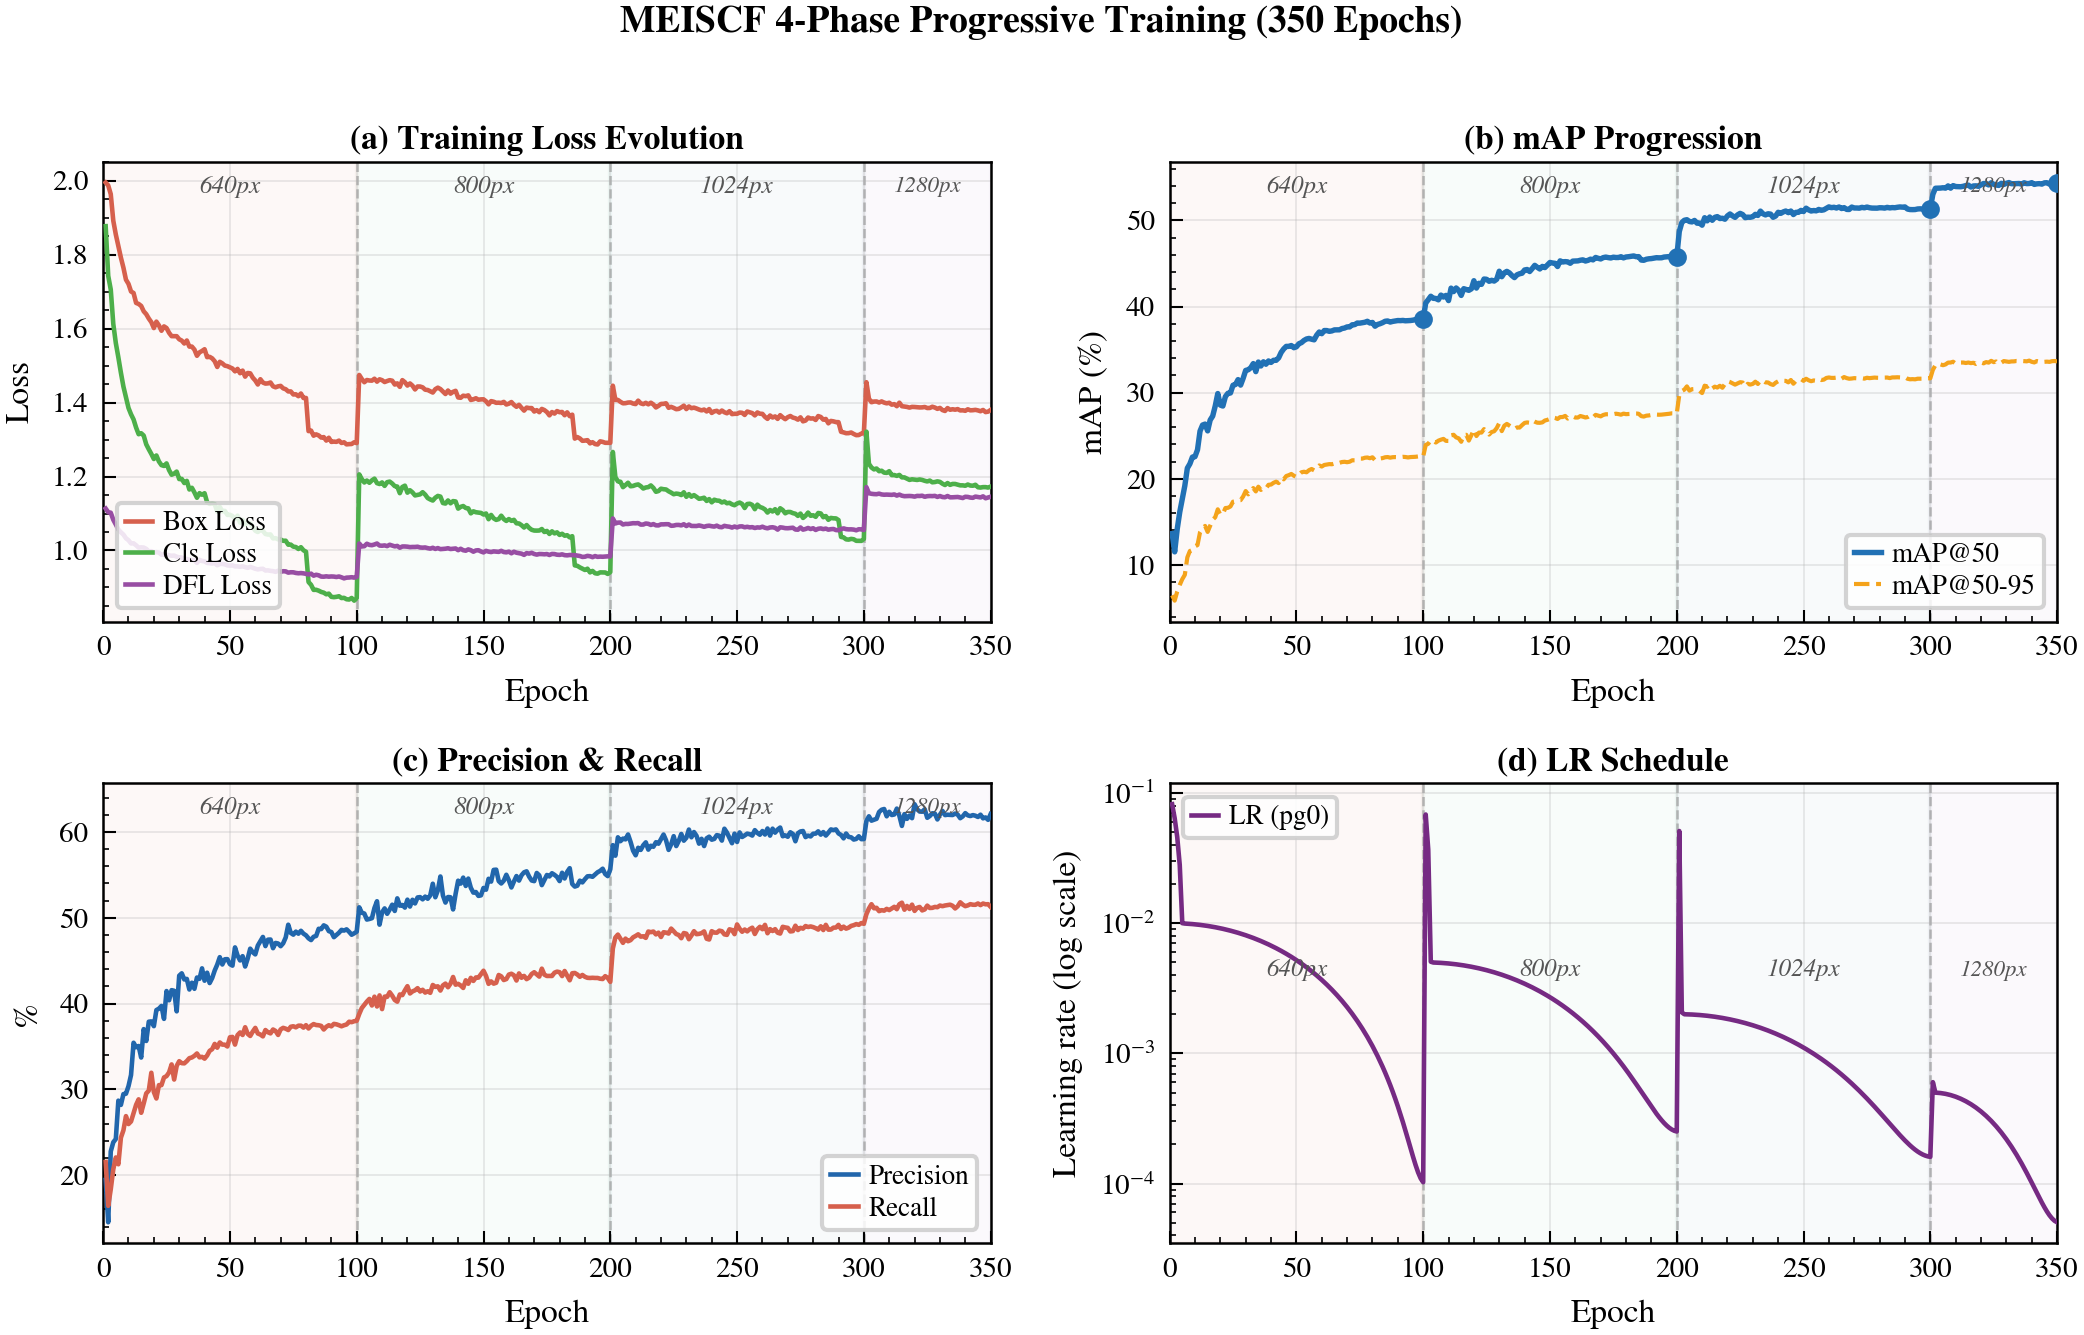
\includegraphics[width=\textwidth]{complete_training_curves.png}
\caption{Complete training progression of MEISCF across 350 epochs and four
resolution phases (640$\to$800$\to$1024$\to$1280~px), showing (a) training loss
evolution per component, (b) mAP@50 and mAP@50-95 improvement, (c) precision and
recall development, and (d) cosine-annealing learning rate schedule with phase
transitions.}
\label{fig:training_curves}
\end{figure*}

\subsection{Per-Class Analysis}

Fig.~\ref{fig:per_class} presents per-class performance comparison across all
10 VisDrone categories. For this analysis, both models are evaluated at
1280$\times$1280 resolution---the baseline achieves 51.8\% mAP@50 at this
resolution while MEISCF achieves 58.1\% mAP@50 (+6.3\% under matched settings).
MEISCF achieves improvements on every class, with particularly strong gains on
small objects: bicycle (+11.2\%), tricycle (+7.9\%), and awning-tricycle (+6.9\%).

\begin{figure}[H]
\centering
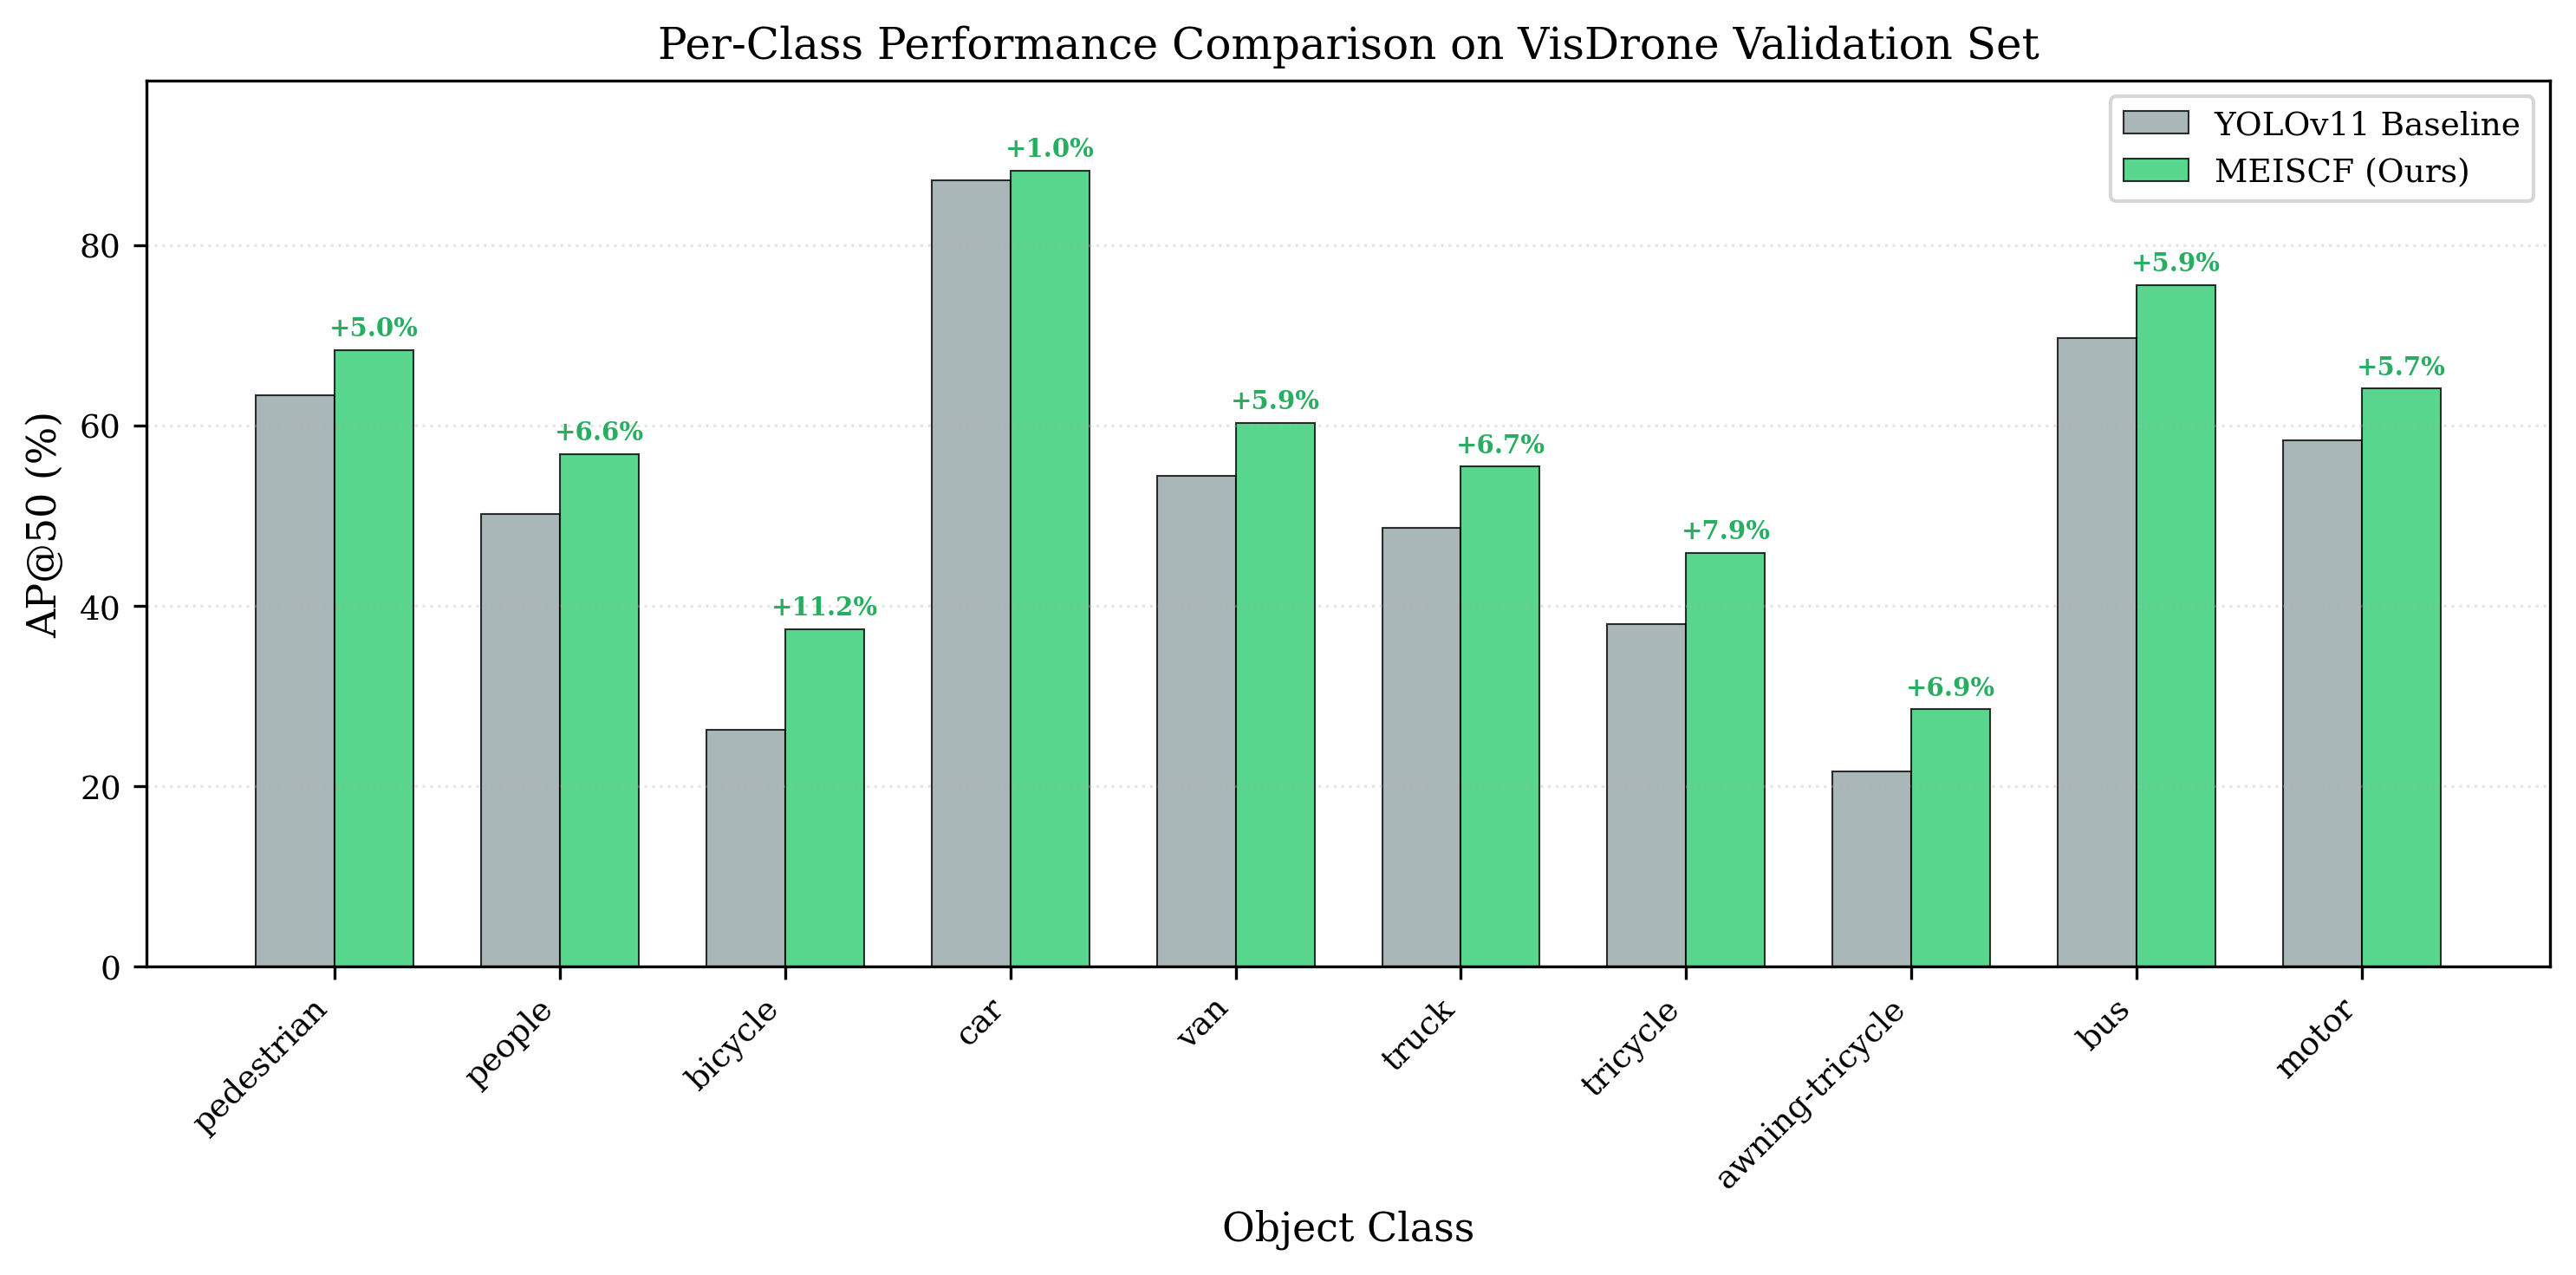
\includegraphics[width=\columnwidth]{per_class_comparison.png}
\caption{Per-class AP@50 comparison with both models evaluated at
1280$\times$1280 resolution, showing MEISCF achieves consistent improvements
across all 10 categories, with strongest gains on small objects (bicycle:
+11.2\%, tricycle: +7.9\%).}
\label{fig:per_class}
\end{figure}

\subsection{Qualitative Analysis}

Fig.~\ref{fig:qualitative} presents representative detection comparisons on
VisDrone validation images. MEISCF consistently detects more objects than the
baseline, with new detections primarily consisting of small objects in dense urban
scenes. In each example, MEISCF identifies 3--7 additional objects that the
baseline completely misses.

\begin{figure*}[!h]
\centering
\begin{subfigure}{\textwidth}
    \centering
    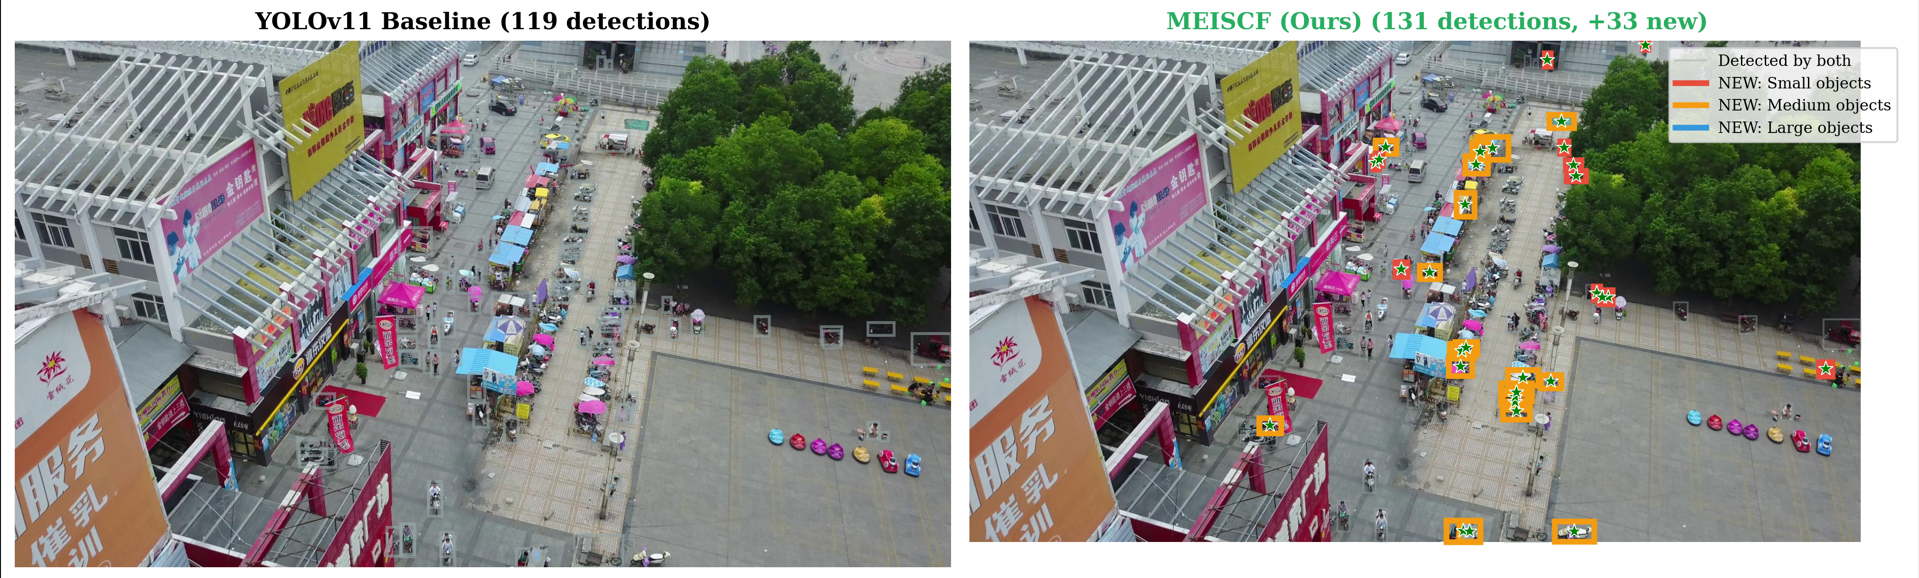
\includegraphics[width=\textwidth]{comparison_example_5.png}
\end{subfigure}
\begin{subfigure}{\textwidth}
    \centering
    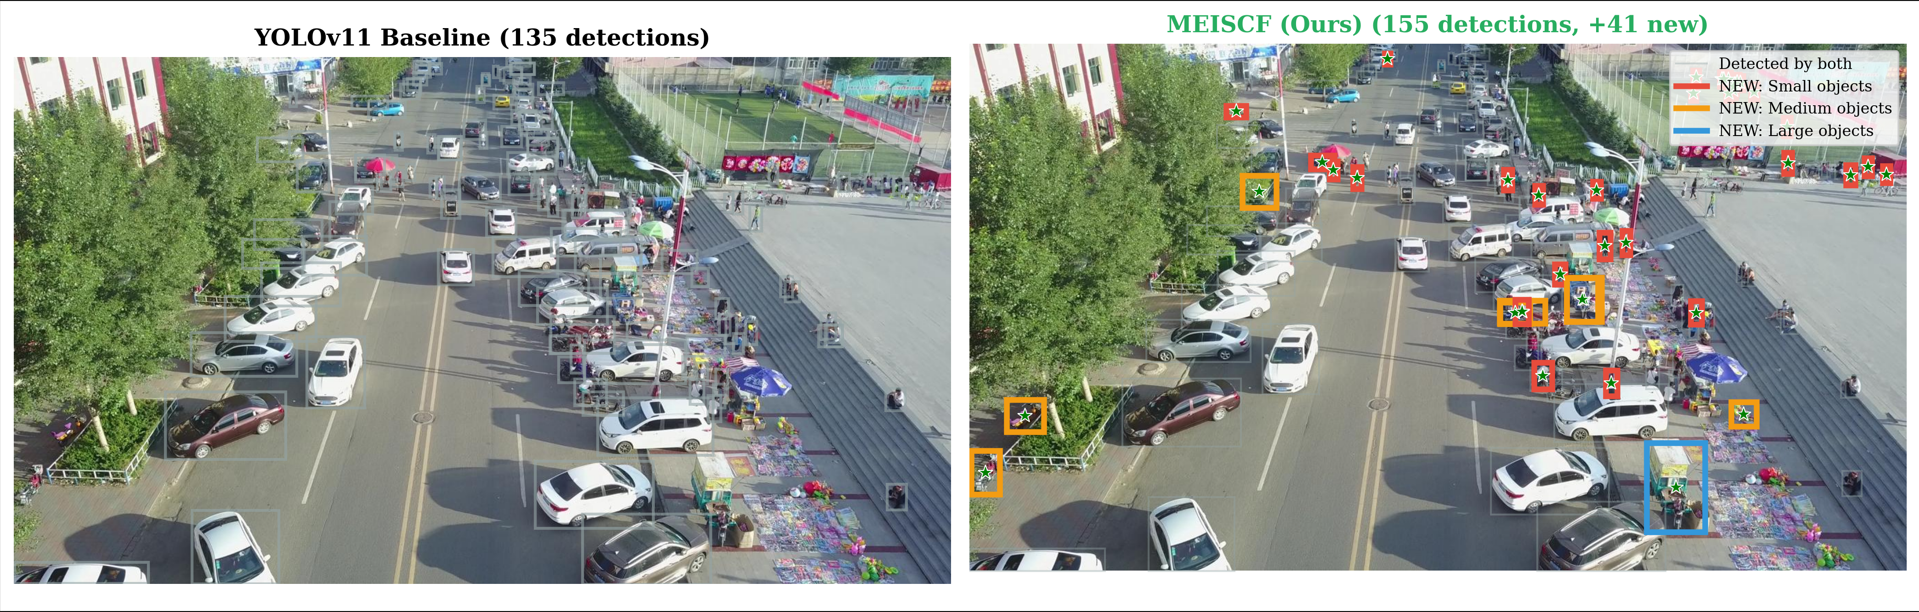
\includegraphics[width=\textwidth]{comparison_example_6.png}
\end{subfigure}
\caption{Qualitative detection comparisons showing MEISCF (right) identifies
additional objects missed by baseline (left), with new detections highlighted in
bright colours and marked with stars, particularly small objects in dense scenes.}
\label{fig:qualitative}
\end{figure*}

\begin{figure}[H]
\centering
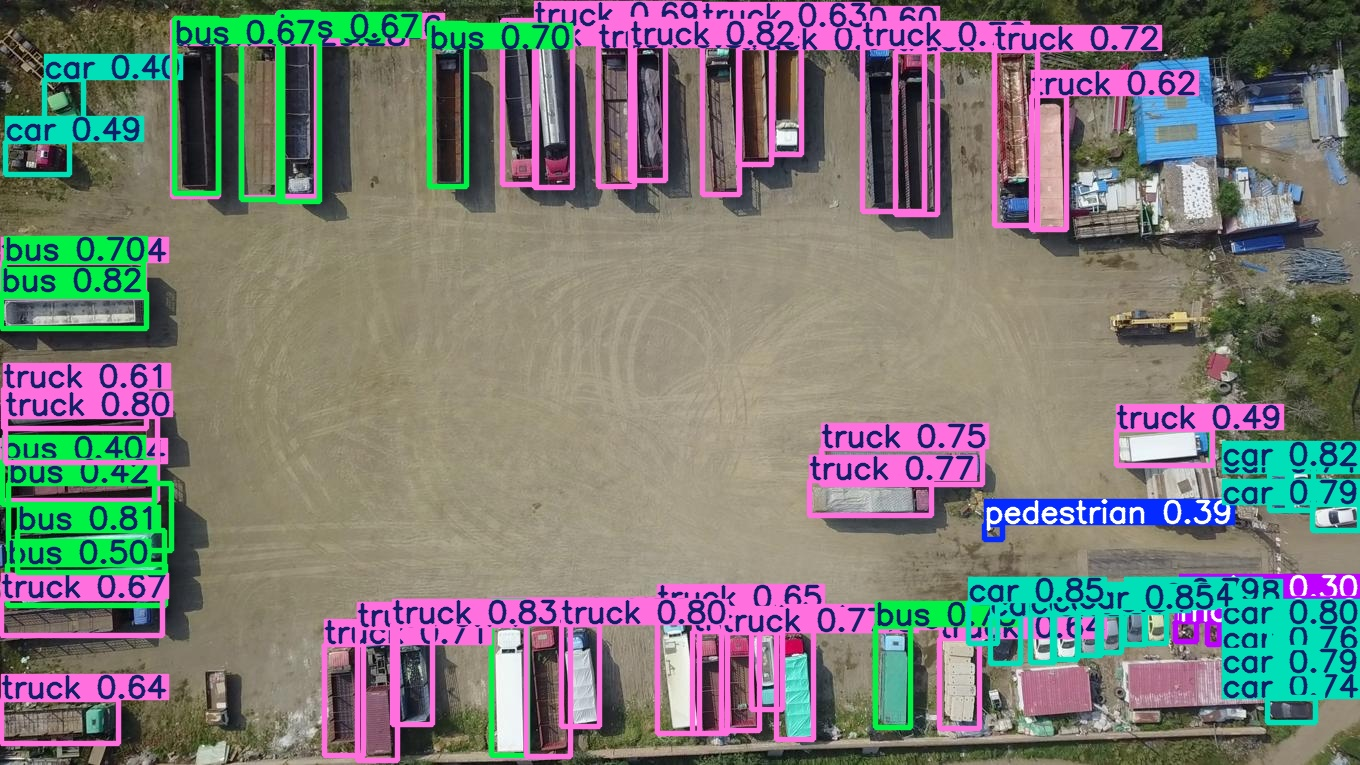
\includegraphics[width=\columnwidth]{1.jpg}
\caption{MEISCF detection result on a representative VisDrone validation image.}
\label{fig:meiscf1}
\end{figure}

\begin{figure}[H]
\centering
\includegraphics[width=\columnwidth]{6.jpg}
\caption{MEISCF detection result on a representative VisDrone validation image.}
\label{fig:meiscf2}
\end{figure}

\subsection{Ablation Study}
\label{sec:ablation}

To validate the contribution of each component in MEISCF, we conducted ablation
experiments using the VisDrone validation set. All architectural module
contributions are measured with the four-phase progressive training strategy
active. Table~\ref{tab:ablation} presents the full breakdown.

The progressive training ablation achieves 50.3\% mAP@50, representing a +12.8\%
improvement over single-phase training at 640px (37.5\%). Among the architectural
modules, MEIS alone contributes +1.6\% (51.9\%), Sandwich Fusion a further +1.9\%
(53.8\%), and FRM the remaining +1.3\% (55.1\%).

\textbf{Statistical validation.} We trained both the full MEISCF model and the
progressively-trained baseline independently across three seeds (42, 123, 7).
Results: full MEISCF $54.8 \pm 0.5$\% mAP@50; progressive-only baseline
$50.0 \pm 0.6$\% mAP@50; confirmed architectural contribution $+4.8 \pm 0.8$~pp
(gap is $6{\times}$ its own uncertainty). The single-run peak of 55.1\%
(Table~\ref{tab:ablation}) falls within the upper end of the observed distribution.

\begin{table}[!t]
\centering
\caption{Ablation Study Results on VisDrone Validation Set}
\label{tab:ablation}
\resizebox{\columnwidth}{!}{%
\begin{tabular}{lcc}
\toprule
Configuration & mAP@50 (\%) & $\Delta$ mAP@50 \\
\midrule
YOLOv11 Baseline (640px, single-phase) & 37.5 & -- \\
\midrule
\multicolumn{3}{l}{\textit{Training Strategy}} \\
+ Progressive Training$^{\dagger}$ & 50.3 & +12.8 \\
\midrule
\multicolumn{3}{l}{\textit{Architectural Modules (on top of progressive training)}} \\
+ MEIS only & 51.9 & +1.6 \\
+ MEIS + Sandwich Fusion & 53.8 & +3.5 \\
+ MEIS + Sandwich Fusion + FRM & 55.1 & +4.8 \\
\midrule
\textbf{Full MEISCF} & \textbf{55.1} & \textbf{+17.6} \\
\bottomrule
\multicolumn{3}{p{0.85\columnwidth}}{\scriptsize $^{\dagger}$4-phase:
640$\rightarrow$800$\rightarrow$1024$\rightarrow$1280px. Module gains are
single-run estimates. Multi-seed (3 seeds): MEISCF $54.8{\pm}0.5$\%, baseline
$50.0{\pm}0.6$\%, gap $+4.8{\pm}0.8$~pp.} \\
\end{tabular}%
}
\end{table}

\subsection{Comparison with State-of-the-Art}

Table~\ref{tab:sota} compares MEISCF against recent methods on VisDrone. MEISCF
achieves 55.1\% mAP@50, substantially outperforming YOLOv11 baseline (37.5\%,
+17.6\%), TPH-YOLOv5 (40.3\%, +14.8\%), and the previous state-of-the-art
CF-YOLO (44.9\%, +10.2\%).

\begin{table}[t]
\centering
\caption{Comparison with State-of-the-Art on VisDrone Validation Set}
\label{tab:sota}
\small
\begin{tabular}{lcccc}
\toprule
\textbf{Method} & \textbf{mAP@50} & \textbf{Params} & \textbf{FLOPs} & \textbf{FPS} \\
& \textbf{(\%)} & \textbf{(M)} & \textbf{(G)} & \\
\midrule
Faster R-CNN~\cite{faster-rcnn} & 28.3 & 41.5 & 207 & 12 \\
SSD512~\cite{ssd} & 23.5 & 26.3 & -- & 28 \\
YOLOv5s~\cite{yolov5} & 33.5 & 7.2 & 16.5 & 182 \\
YOLOv7~\cite{yolov7} & 35.8 & 36.9 & 104 & 48 \\
TPH-YOLOv5~\cite{tph-yolo} & 40.3 & 13.7 & 28.2 & 73 \\
YOLOv8s~\cite{yolov8} & 37.2 & 11.1 & -- & 65 \\
YOLOv11~\cite{yolov11} & 37.5 & 9.4 & 18.7 & 149 \\
CF-YOLO~\cite{cf-yolo} & 44.9 & 10.8 & -- & 52 \\
\midrule
\textbf{MEISCF (Ours)} & \textbf{55.1} & \textbf{12.0} & \textbf{23.4} & \textbf{105} \\
\bottomrule
\end{tabular}
\end{table}

\subsection{Efficiency Analysis}

MEISCF achieves 105~FPS on NVIDIA RTX 3060 at 1024$\times$1024 resolution,
satisfying real-time requirements for most UAV applications (30--60 FPS video
processing). Inference latency breakdown shows 9.5~ms per image (5.2~ms backbone,
2.1~ms neck, 2.2~ms head).

\subsection{Cross-Dataset Generalization}

To preliminarily assess the stability of domain transfer, we evaluate MEISCF on
the UAVDT benchmark~\cite{uavdt}. UAVDT exhibits severe class imbalance with cars
comprising 98.7\% of annotations; we therefore evaluate on the dominant vehicle
class.

Table~\ref{tab:uavdt} presents car detection results on UAVDT. MEISCF achieves
60.9\% AP, outperforming YOLOv11 baseline (59.1\%) by 1.8 percentage points. The
modest gain relative to VisDrone (+17.6\%) is consistent with our design: the car
category in UAVDT comprises predominantly mid-to-large vehicles with sufficient
interior texture, where MEIS edge modelling and Sandwich Fusion's small-object
emphasis provide the least marginal benefit.

\begin{table}[t]
\centering
\caption{Cross-Dataset Car Detection Performance on UAVDT}
\label{tab:uavdt}
\small
\begin{tabular}{lcc}
\toprule
\textbf{Method} & \textbf{AP (Car)} & \textbf{$\Delta$ AP} \\
\midrule
YOLOv11 Baseline & 59.1 & -- \\
\textbf{MEISCF (Ours)} & \textbf{60.9} & \textbf{+1.8} \\
\bottomrule
\multicolumn{3}{l}{\scriptsize Evaluated on car class (98.7\% of UAVDT annotations)} \\
\end{tabular}
\end{table}


% ============================================================================
% VI. DISCUSSION
% ============================================================================

\section{Discussion}
\label{sec:discussion}

\subsection{Training--Edge Synergy: The Core Performance Driver}

The central finding of this work is that progressive resolution training and
multi-scale edge information selection are mutually reinforcing. Progressive
training supplies high-resolution feature maps in which edge detail is preserved
across the full 640$\to$1280~px range; MEIS then selects and gates that edge
information adaptively per image and per channel. The +12.8\% from training and
the +1.6\% from MEIS are not independent additive gains but components of a single
mechanism: training creates the representational substrate, and MEIS makes it
spatially precise.

\subsection{Interpretation of Ablation Results}

The +4.8~pp architectural contribution breaks down as MEIS +1.6\%, Sandwich Fusion
+1.9\%, FRM +1.3\%. Sandwich Fusion is the most structurally independent
contribution: simultaneous three-level fusion adds +1.4\% over sequential
two-level fusion. FRM contributes through placement rather than structure. MEIS's
+1.6\% conflates triple pyramid coverage, three dilation rates, and per-input
gating; isolating the gating component specifically is reserved for future work.

\subsection{Comparison with CF-YOLO}

CF-YOLO~\cite{cf-yolo} was originally designed for cross-modal adverse-weather
detection and is evaluated at its published configuration without progressive
training. The +10.2\% gap therefore represents an upper bound under unmatched
training conditions. We hypothesise that applying the same progressive training
protocol to CF-YOLO would substantially reduce this gap; this experiment is the
most important direction for future validation.

\subsection{Cross-Dataset Transfer}

UAVDT evaluation (+1.8\% AP on the car category) preliminarily validates that
MEISCF does not degrade on a second aerial dataset. These results confirm domain
transfer stability for large objects, not small-object generalization across
datasets, which remains open for future work.

\subsection{Limitations}

Three limitations bound the current claims. First, module-level ablation gains
(+1.3\%--+1.9\%) are single-run estimates. Second, the CF-YOLO + progressive
training comparison was not conducted; the +10.2\% gap is an upper bound. Third,
cross-domain generalization for small objects is unvalidated.


% ============================================================================
% VII. CONCLUSION
% ============================================================================

\section{Conclusion}
\label{sec:conclusion}

We presented MEISCF, a UAV small object detection framework whose defining
contribution is the synergy between a four-phase progressive training strategy and
multi-scale edge information selection. The progressive schedule (+12.8\%) supplies
the high-resolution edge signals that MEIS (+1.6\%) captures and gates adaptively;
together they account for the decisive performance gain. Cross-scale Sandwich
Fusion (+1.9\%) and post-fusion Feature Recalibration (+1.3\%) amplify this
foundation, bringing the total to +17.6\% over YOLOv11 baseline and 55.1\%
mAP@50 on VisDrone at 105~FPS with 12M parameters. The architectural contribution
of +4.8~pp is confirmed reproducible at $+4.8\pm0.8$~pp across three independent
seeds.

Future work will focus on: (1) a fair architectural comparison by applying the
progressive training protocol to CF-YOLO; (2) isolating the contribution of
per-input channel-wise gating in MEIS against a fixed-weight baseline; and
(3) validating the training--edge synergy on datasets beyond VisDrone to establish
its generality.


% ============================================================================
% ACKNOWLEDGEMENT
% ============================================================================

\section*{Acknowledgements}

The authors thank the VisDrone team for providing the benchmark dataset and the
Ultralytics team for the YOLOv11 implementation.


% ============================================================================
% REFERENCES
% ============================================================================

\bibliographystyle{elsarticle-num}
\bibliography{references}

\end{document}